% Artigo formatado diretamente com o template oficial da SBC.

\documentclass[12pt]{article}
\usepackage{sbc-template}

% ----------------------------------------------------------------
% Idioma e codificação
% ----------------------------------------------------------------
\usepackage[T1]{fontenc}
\usepackage[utf8]{inputenc}
\usepackage[brazil,english]{babel}

% ----------------------------------------------------------------
% Matemática e microtipografia
% ----------------------------------------------------------------
\usepackage{amsmath}
\usepackage{microtype}

% ----------------------------------------------------------------
% Figuras, tabelas, links e legendas
% ----------------------------------------------------------------
\usepackage{graphicx}
\graphicspath{{assets/}}
\newcommand{\thesisfiguregraphic}[1]{%
    \includegraphics[width=\textwidth,height=0.78\textheight,keepaspectratio]{#1}%
}
\usepackage{array}
\usepackage{booktabs}
\usepackage{xcolor}
\usepackage{pifont}
\usepackage{url}
\usepackage[hidelinks]{hyperref}


\usepackage{tabularx}
\usepackage{longtable}
\usepackage{array}
\usepackage{float}
\newcolumntype{Y}{>{\raggedright\arraybackslash}X}
\newcolumntype{L}[1]{>{\raggedright\arraybackslash}p{#1}}
\newcolumntype{C}[1]{>{\centering\arraybackslash}p{#1}}
\newcommand{\codebreak}[1]{{\footnotesize\ttfamily #1}}
\newcommand{\codemath}[1]{\mbox{\footnotesize\ttfamily #1}}
\newcommand{\statusyes}{\textcolor{green!50!black}{\ding{51}}}
\newcommand{\statusno}{\textcolor{red!70!black}{\ding{55}}}
\newcommand{\statuspositive}[1]{\statusyes~#1}
\newcommand{\statuspartial}[1]{\textcolor{orange!85!black}{\ding{108}}~#1}
\newcommand{\statusvalidated}{\textcolor{green!50!black}{\ding{51}}}
\newcommand{\statusexperimental}{\textcolor{orange!85!black}{\ding{108}}}
\newcommand{\statusproposed}{\textcolor{blue!70!black}{\ding{117}}}
\setlength{\emergencystretch}{3em}
\usepackage{tikz}
\usetikzlibrary{arrows.meta, positioning, fit, calc, shapes.geometric}
\newcommand{\serverglyph}[1]{%
\begin{scope}[shift={#1}]
  \draw[fill=gray!20, rounded corners=1pt] (0,0) rectangle (0.36,0.62);
  \draw[fill=gray!35] (0.36,0) -- (0.52,0.10) -- (0.52,0.72) -- (0.36,0.62) -- cycle;
  \draw (0.07,0.46) -- (0.28,0.46);
  \draw (0.07,0.34) -- (0.28,0.34);
  \draw (0.07,0.22) -- (0.20,0.22);
  \fill (0.09,0.09) circle (0.025);
\end{scope}}

\newcommand{\dbglyph}[1]{%
\begin{scope}[shift={#1}]
  \draw[fill=gray!20] (0,0) ellipse (0.34 and 0.11);
  \draw[fill=gray!12] (-0.34,0) -- (-0.34,-0.55) arc (180:360:0.34 and 0.11) -- (0.34,0);
  \draw (0,-0.18) ellipse (0.34 and 0.11);
  \draw (0,-0.37) ellipse (0.34 and 0.11);
\end{scope}}

\newcommand{\personglyph}[1]{%
\begin{scope}[shift={#1}]
  \draw[fill=gray!10] (0,0) circle (0.34);
  \fill[gray!55] (0,0.12) circle (0.11);
  \draw[fill=gray!45] (-0.18,-0.18) arc (180:0:0.18 and 0.17) -- (0.18,-0.28) -- (-0.18,-0.28) -- cycle;
\end{scope}}

\newcommand{\thesisprismatikz}{%
\begin{figure}[H]
\centering
\resizebox{0.74\textwidth}{!}{%
\begin{tikzpicture}[
  box/.style={rectangle, draw, very thick, minimum width=9.2cm, minimum height=1.55cm, align=center, font=\large},
  arrow/.style={-{Latex[length=4mm]}, line width=1.2pt},
  node distance=0.72cm
]
\node[font=\bfseries\LARGE] (title) {PRISMA Flow Diagram};
\node[box, below=0.85cm of title] (id) {Identification\\{\normalsize 2581 records retrieved}};
\node[box, below=of id] (screen) {Screening\\{\normalsize 5 duplicates removed}\\{\normalsize 2576 records screened}};
\node[box, below=of screen] (elig) {Eligibility\\{\normalsize 2559 excluded}\\{\normalsize 17 full-text assessed}};
\node[box, below=of elig] (inc) {Included\\{\normalsize 6 studies in final review}};
\draw[arrow] (id) -- (screen);
\draw[arrow] (screen) -- (elig);
\draw[arrow] (elig) -- (inc);
\end{tikzpicture}}
\caption{PRISMA flow diagram.}
\end{figure}}

\newcommand{\thesislayerstikz}{%
\begin{figure}[H]
\centering
\resizebox{0.92\textwidth}{!}{%
\begin{tikzpicture}[
  baseLayer/.style={rectangle, rounded corners=6pt, very thick, minimum width=10.5cm, minimum height=1.55cm, text width=10cm, align=center},
  appLayer/.style={baseLayer, draw=orange!70!black, fill=orange!18},
  serviceLayer/.style={baseLayer, draw=blue!70!black, fill=blue!18},
  overlayLayer/.style={baseLayer, draw=green!70!black, fill=green!18},
  physicalLayer/.style={baseLayer, draw=gray!70!black, fill=gray!18},
  label/.style={font=\bfseries, align=right, text width=2.35cm},
  node distance=0.42cm
]
\node[appLayer] (app) {\textbf{Application Layer}\\[2pt]Decentralized Applications \quad Social Network\\File Sharing \quad DApps};
\node[serviceLayer, below=of app] (svc) {\textbf{Service Layer}\\[2pt]Secure Messaging \quad Data Access Services \quad Session Management};
\node[overlayLayer, below=of svc] (ovl) {\textbf{Overlay Network Layer}\\[2pt]Peer Discovery \quad Routing \& Anonymity \quad Distributed Storage};
\node[physicalLayer, below=of ovl] (phy) {\textbf{Physical \& Classical Network Layer}\\[2pt]IP / UDP / TCP / QUIC \quad NAT Traversal \quad STUN / TURN / Relay};
\node[label, left=0.8cm of app] {Application-Level};
\node[label, left=0.8cm of svc] {Reusable Services};
\node[label, left=0.8cm of ovl] {Overlay Coordination};
\node[label, left=0.8cm of phy] {Physical Connectivity};
\end{tikzpicture}}
\caption{Layered architecture.}
\label{fig:layered-architecture}
\end{figure}}

\newcommand{\thesisconnectiontikz}{%
\begin{figure}[H]
\centering
\resizebox{0.98\textwidth}{!}{%
\begin{tikzpicture}[
  panel/.style={rectangle, draw, minimum width=2.75cm, minimum height=1.45cm, align=center},
  main/.style={rectangle, draw, rounded corners=5pt, very thick, minimum width=4.25cm, minimum height=0.9cm, align=center, font=\bfseries},
  small/.style={rectangle, draw, minimum width=2.35cm, minimum height=0.62cm, align=center, font=\scriptsize},
  arrow/.style={-{Latex[length=3mm]}, thick},
  dashedlink/.style={dashed, gray!70, thick}
]
\node[font=\bfseries\Large] at (0,4.1) {Connection Management};
\draw (-6.4,3.72) -- (3.35,3.72);
\node[panel] (phys) at (-5.0,2.25) {\textbf{Physical Peers}\\[0.75cm]};
\serverglyph{(-5.45,1.77)} \serverglyph{(-4.65,1.77)}
\node[panel, text width=2.45cm] (meta) at (-5.0,-0.15) {\textbf{Peer Metadata}\\[3pt]\scriptsize endpoints\\reachability\\transport};
\node[main] (cm) at (0,2.25) {Connection Management};
\node[panel, text width=2.45cm] (endpoint) at (5.05,3.0) {\textbf{Endpoint Options}\\[3pt]IPv4\\IPv6\\Relay};
\node[panel, text width=2.45cm] (status) at (5.05,-0.15) {\textbf{Status Check}\\[3pt]Valid\\Degraded\\Failed};
\node[align=left, text width=5.85cm, font=\small] (opts) at (0,0.0) {$\bullet$ Direct Connection\\$\bullet$ Hole Punching / NAT Traversal\\$\bullet$ Relay-Assisted Establishment\\$\bullet$ Continuous Relay Forwarding};
\node[font=\bfseries] (auto) at (0,-2.22) {Automatic Selection};
\node[small] (ka) at (-3.75,-3.55) {Keep-Alive};
\node[small] (fd) at (-1.25,-3.55) {Failure Detection};
\node[small] (ru) at (1.25,-3.55) {Retry \& Update};
\node[small] (rf) at (3.75,-3.55) {Relay Forwarding};
\draw[arrow] (phys.east) -- (cm.west);
\draw[arrow] (cm.east) -- (endpoint.west);
\draw[dashedlink] (phys) -- (meta);
\draw[dashedlink] (cm.east) -- (status.west);
\draw[arrow] (opts.south) -- (auto.north);
\draw[arrow] (auto.south) -- ++(0,-0.45) -| (ka.north);
\draw[arrow] (auto.south) -- ++(0,-0.45) -| (fd.north);
\draw[arrow] (auto.south) -- ++(0,-0.45) -| (ru.north);
\draw[arrow] (auto.south) -- ++(0,-0.45) -| (rf.north);
\end{tikzpicture}}
\caption{Connection Management diagram.}
\end{figure}}

\newcommand{\thesisdrttikz}{%
\begin{figure}[H]
\centering
\resizebox{0.98\textwidth}{!}{%
\begin{tikzpicture}[
  vnode/.style={rectangle, draw=blue!55!black, rounded corners=5pt, fill=blue!8, minimum width=1.9cm, minimum height=0.72cm, align=center},
  pgroup/.style={rectangle, draw=gray!75!black, dashed, rounded corners=8pt, fill=gray!4, minimum width=3.15cm, minimum height=1.18cm, align=center},
  pn/.style={rectangle, draw=gray!70!black, rounded corners=3pt, fill=gray!16, minimum width=1.18cm, minimum height=0.38cm, align=center, font=\scriptsize},
  cell/.style={font=\scriptsize, align=center},
  arrow/.style={-{Latex[length=3mm]}, thick},
  dashedarrow/.style={-{Latex[length=3mm]}, dashed, thick}
]
\node[font=\bfseries\Large] at (0,5.35) {Distributed Routing Table (DRT)};
\node[text width=10.2cm, align=center, font=\small] at (0,4.55) {The DRT indirectly maps a virtual node identifier to physical entry points authorized to receive its traffic.};
\node[align=center] at (-5.85,3.08) {\textbf{Virtual Nodes}\\(logical identities)};
\node[vnode] (v1) at (-5.85,2.05) {$H(pk_1)$};
\node[vnode] (v2) at (-5.85,0.60) {$H(pk_2)$};
\node[vnode] (vn) at (-5.85,-1.10) {$H(pk_n)$};
\node[draw, rounded corners=8pt, fill=gray!5, minimum width=5.75cm, minimum height=3.82cm] (table) at (0,0.45) {};
\node[font=\bfseries] at (0,2.58) {DRT Records};
\draw (-2.55,1.68) rectangle (2.55,-1.02);
\draw (-0.35,1.68) -- (-0.35,-1.02);
\draw (-2.55,1.0) -- (2.55,1.0);
\draw (-2.55,0.32) -- (2.55,0.32);
\draw (-2.55,-0.36) -- (2.55,-0.36);
\node[cell, font=\scriptsize\bfseries] at (-1.45,1.34) {Virtual ID};
\node[cell, font=\scriptsize\bfseries] at (1.10,1.34) {Entry point IDs};
\node[cell] at (-1.45,0.66) {$H(pk_1)$};
\node[cell] at (1.10,0.66) {$\{pn_a,\ pn_b\}$};
\node[cell] at (-1.45,-0.02) {$H(pk_2)$};
\node[cell] at (1.10,-0.02) {$\{pn_c,\ pn_d\}$};
\node[cell] at (-1.45,-0.70) {$H(pk_n)$};
\node[cell] at (1.10,-0.70) {$\{pn_x,\ ...\}$};
\node[align=center] at (5.75,3.08) {\textbf{Physical Nodes}\\(entry points)};
\node[pgroup] (p1) at (5.75,1.90) {};
\node[pn] at (5.10,2.08) {$pn_a$};
\node[pn] at (6.40,2.08) {$pn_b$};
\node[cell] at (5.75,1.60) {authorized for $H(pk_1)$};
\node[pgroup] (p2) at (5.75,0.40) {};
\node[pn] at (5.10,0.58) {$pn_c$};
\node[pn] at (6.40,0.58) {$pn_d$};
\node[cell] at (5.75,0.10) {authorized for $H(pk_2)$};
\node[pgroup] (p3) at (5.75,-1.10) {};
\node[pn] at (5.10,-0.92) {$pn_x$};
\node[pn] at (6.40,-0.92) {$...$};
\node[cell] at (5.75,-1.40) {authorized for $H(pk_n)$};
\draw[dashedarrow] (v1.east) -- (table.west |- v1);
\draw[dashedarrow] (v2.east) -- (table.west |- v2);
\draw[dashedarrow] (vn.east) -- (table.west |- vn);
\draw[arrow] (table.east |- p1) -- (p1.west);
\draw[arrow] (table.east |- p2) -- (p2.west);
\draw[arrow] (table.east |- p3) -- (p3.west);
\node[draw, rounded corners=5pt, text width=10.2cm, align=left, fill=blue!4, font=\small] at (0,-3.35) {$\bullet$ The DRT does not store complete routes.\\$\bullet$ It provides authorized physical entry points.\\$\bullet$ Virtual-to-physical mapping remains indirect.};
\end{tikzpicture}}
\caption{Distributed Routing Table.}
\end{figure}}

\newcommand{\thesishopbyhoptikz}{%
\begin{figure}[H]
\centering
\resizebox{0.98\textwidth}{!}{%
\begin{tikzpicture}[
  hop/.style={rectangle, draw=gray!75!black, rounded corners=5pt, fill=gray!10, minimum width=1.45cm, minimum height=0.74cm, align=center, font=\scriptsize},
  vnode/.style={rectangle, draw=blue!60!black, rounded corners=6pt, fill=blue!8, minimum width=1.7cm, minimum height=0.78cm, align=center, font=\scriptsize},
  finalnode/.style={rectangle, draw=red!65!black, rounded corners=6pt, fill=red!6, minimum width=1.65cm, minimum height=0.78cm, align=center, font=\scriptsize},
  route/.style={-{Latex[length=3mm]}, very thick, blue!65!black},
  alt/.style={-{Latex[length=2.6mm]}, dashed, thick, gray!70},
  note/.style={font=\scriptsize, align=center, fill=white, inner sep=1.5pt}
]
\node[font=\bfseries\Large] at (0,5.45) {TTL-Based Hop-by-Hop Route Example};
\node[text width=10.1cm, align=center, font=\small] at (0,4.45) {A route is built incrementally: each physical node stores only its local mapping and chooses the next hop while TTL remains valid.};
\node[vnode] (vn) at (-5.85,2.45) {VN\\request};
\node[hop] (entry) at (-3.55,2.45) {Entry PN\\TTL 4};
\node[hop] (hop1) at (-1.25,2.45) {Hop 1\\TTL 3};
\node[hop] (hop2) at (1.05,2.45) {Hop 2\\TTL 2};
\node[hop] (hop3) at (3.35,2.45) {Hop 3\\TTL 1};
\node[finalnode] (final) at (5.65,2.45) {Final PN\\TTL 0};
\draw[route] (vn.east) -- (entry.west);
\draw[route] (entry.east) -- (hop1.west);
\draw[route] (hop1.east) -- (hop2.west);
\draw[route] (hop2.east) -- (hop3.west);
\draw[route] (hop3.east) -- (final.west);
\node[note] at (-4.70,2.90) {entry};
\node[note] at (-2.40,2.90) {random next};
\node[note] at (-0.10,2.90) {random next};
\node[note] at (2.20,2.90) {random next};
\node[note, text=red!70!black] at (4.50,2.90) {TTL ends};
\node[draw=blue!60!black, rounded corners=5pt, fill=blue!5, align=center, font=\scriptsize, text width=3.0cm] at (-3.45,1.05) {Each hop saves only\\previous $\rightarrow$ next};
\node[draw=blue!60!black, rounded corners=5pt, fill=blue!5, align=center, font=\scriptsize, text width=3.0cm] at (0,1.05) {TTL decreases\\at every hop};
\node[draw=red!65!black, rounded corners=5pt, fill=red!5, align=center, font=\scriptsize, text width=3.0cm] at (3.45,1.05) {Construction finishes\\at the final PN};
\draw[alt] (-3.45,0.25) .. controls (-1.25,-0.42) and (1.25,-0.42) .. (3.45,0.25);
\node[note] at (0,-0.40) {another random walk can build a different path};
\node[draw, rounded corners=5pt, fill=blue!4, text width=10.2cm, align=left, font=\small] at (0,-2.25) {$\bullet$ Each hop chooses one next physical node.\\$\bullet$ TTL decreases at every forwarding step.\\$\bullet$ The route emerges during forwarding.};
\end{tikzpicture}}
\caption{Example of hop-by-hop route construction with a TTL-based strategy.}
\label{fig:ttl-route-strategy-example}
\end{figure}}

\newcommand{\thesisroutestrategyconstructiontikz}{%
\begin{figure}[H]
\centering
\resizebox{0.98\textwidth}{!}{%
\begin{tikzpicture}[
  block/.style={rectangle, draw=gray!75!black, rounded corners=6pt, fill=gray!8, minimum width=2.05cm, minimum height=0.72cm, align=center, font=\scriptsize},
  protocol/.style={rectangle, draw=blue!65!black, rounded corners=7pt, fill=blue!8, minimum width=2.75cm, minimum height=0.88cm, align=center, font=\scriptsize},
  strategy/.style={rectangle, draw=orange!75!black, rounded corners=7pt, fill=orange!10, minimum width=2.75cm, minimum height=0.88cm, align=center, font=\scriptsize},
  hop/.style={circle, draw=gray!70!black, fill=gray!8, minimum size=0.88cm, align=center, font=\scriptsize},
  finalnode/.style={circle, draw=red!65!black, fill=red!8, minimum size=0.98cm, align=center, font=\scriptsize},
  record/.style={rectangle, draw=purple!65!black, rounded corners=5pt, fill=purple!7, minimum width=2.45cm, minimum height=0.68cm, align=center, font=\scriptsize},
  arrow/.style={-{Latex[length=2.8mm]}, thick, blue!65!black},
  control/.style={-{Latex[length=2.5mm]}, thick, orange!80!black},
  dashedarrow/.style={-{Latex[length=2.5mm]}, dashed, thick, gray!70},
  note/.style={font=\scriptsize, align=center, fill=white, inner sep=1.2pt}
]
\node[font=\bfseries\Large] at (0,5.70) {Strategy-Based Route Construction};
\node[text width=11.6cm, align=center, font=\small] at (0,4.72) {The route protocol keeps the lifecycle stable. The active route strategy chooses each next physical hop and defines when construction should finish.};

\node[block, fill=green!8, draw=green!45!black] (vn) at (-5.35,3.10) {Virtual node\\requests route};
\node[protocol] (protocol) at (-2.55,3.10) {Route protocol\\lifecycle};
\node[strategy] (strategy) at (0.45,3.10) {Route strategy\\policy};
\node[block, fill=blue!6, draw=blue!55!black] (mapping) at (3.25,3.10) {Local mappings\\per hop};
\node[record, minimum width=2.15cm] (drt) at (6.05,3.10) {DRT entry\\published};

\draw[arrow] (vn.east) -- (protocol.west);
\draw[arrow] (protocol.east) -- (strategy.west);
\draw[arrow] (strategy.east) -- (mapping.west);
\draw[arrow] (mapping.east) -- (drt.west);

\node[hop] (h1) at (-4.45,1.30) {PN};
\node[hop] (h2) at (-2.20,1.30) {PN};
\node[hop] (h3) at (0.05,1.30) {PN};
\node[hop] (h4) at (2.30,1.30) {PN};
\node[finalnode] (final) at (4.55,1.30) {Final\\PN};

\draw[arrow] (h1.east) -- node[note, above=3pt, font=\tiny] {\texttt{path\_id}} (h2.west);
\draw[arrow] (h2.east) -- node[note, above=3pt, font=\tiny] {\texttt{path\_id}} (h3.west);
\draw[arrow] (h3.east) -- node[note, above=3pt, font=\tiny] {\texttt{path\_id}} (h4.west);
\draw[arrow] (h4.east) -- node[note, above=3pt, font=\tiny] {\texttt{path\_id}} (final.west);

\draw[control] (strategy.south) -- ++(0,-0.55) -| node[pos=0.28, right, note] {next-hop choice} (h3.north);
\draw[dashedarrow] (final.north) -- ++(0,0.55) -| (drt.south);

\node[record, text width=2.40cm] (candidates) at (-4.00,-0.35) {Candidate peers\\and local state};
\node[record, text width=2.65cm] (objectives) at (-0.55,-0.35) {Optimization goal\\privacy / latency\\bandwidth / reliability};
\node[record, text width=2.40cm] (termination) at (2.90,-0.35) {Termination rule\\strategy-specific};

\node[draw, rounded corners=5pt, fill=blue!4, text width=11.0cm, align=left, font=\small] at (0,-2.62) {$\bullet$ The protocol defines invariant route lifecycle messages and publication rules.\\$\bullet$ The strategy defines hop selection and stopping conditions.\\$\bullet$ Different strategies can optimize privacy, latency, bandwidth, reliability, or diversity without changing route execution.};
\end{tikzpicture}}
\caption{Generic route construction through a route strategy.}
\end{figure}}

\newcommand{\thesispeerdiscoverytikz}{%
\begin{figure}[H]
\centering
\resizebox{0.96\textwidth}{!}{%
\begin{tikzpicture}[
  arrow/.style={-{Latex[length=2.8mm]}, thick, blue!65!black},
  dashedarrow/.style={-{Latex[length=2.5mm]}, dashed, thick, gray!70},
  seed/.style={rectangle, draw=green!45!black, rounded corners=4pt, fill=green!8, minimum width=2.38cm, minimum height=0.58cm, align=center, font=\scriptsize},
  public/.style={circle, draw=blue!60!black, fill=blue!8, minimum size=0.9cm, align=center, font=\scriptsize},
  private/.style={circle, draw=red!60!black, fill=red!7, minimum size=0.9cm, align=center, font=\scriptsize},
  box/.style={rectangle, draw=gray!75!black, rounded corners=5pt, fill=gray!8, minimum width=2.35cm, minimum height=0.78cm, align=center, font=\scriptsize},
  relay/.style={diamond, draw=orange!70!black, fill=orange!10, aspect=1.6, inner sep=1.5pt, minimum width=1.55cm, minimum height=1.0cm, align=center, font=\scriptsize},
  meta/.style={rectangle, draw=purple!55!black, rounded corners=5pt, fill=purple!7, minimum width=2.85cm, minimum height=0.78cm, text width=2.65cm, align=center, font=\scriptsize},
  stage/.style={font=\bfseries\scriptsize, align=center, text width=2.55cm}
]
\node[font=\bfseries\Large] at (0,5.85) {Peer Discovery Process};
\node[text width=13.0cm, align=center, font=\small] at (0,4.82) {Public peers bootstrap the network, learn about private peers, and share reachability metadata for relay or hole-punch attempts.};

\node[stage] at (-5.55,3.78) {1. Bootstrap};
\node[seed] (seed1) at (-5.55,2.92) {DNS seeds};
\node[seed] (seed2) at (-5.55,2.05) {Hardcoded\\public nodes};

\node[stage] at (-2.55,3.78) {2. Public peer view};
\node[public] (pubA) at (-3.25,2.68) {P1};
\node[public] (pubB) at (-1.85,2.68) {P2};
\node[public] (pubC) at (-2.55,1.65) {P3};
\node[box, fill=blue!6, draw=blue!50!black, minimum width=2.75cm] (publicView) at (-2.55,0.35) {Known public\\peer exchange};
\draw[dashed, gray!65] (pubA) -- (pubB) -- (pubC) -- (pubA);

\node[stage] at (0.90,3.78) {3. Private peers};
\node[box, draw=red!55!black, fill=red!4, minimum width=3.05cm,
      minimum height=1.85cm] (nat) at (0.90,2.05) {};
\node[private] (privA) at (0.20,2.30) {N1};
\node[private] (privB) at (1.60,2.30) {N2};
\node[font=\scriptsize] at (0.90,1.43) {Behind NAT / Firewall};

\node[stage] at (4.85,3.78) {4. Connect};
\node[meta] (meta) at (4.85,2.45) {Published metadata\\reachable via relay\\or hole punching};
\node[relay] (relay) at (3.82,0.62) {Relay};
\node[box, fill=orange!7, draw=orange!70!black] (hole) at (5.88,0.62) {Hole punching\\attempt};
\node[public] (newPeer) at (4.85,-0.72) {P4};

\draw[arrow] (seed1.east) -- (pubA.west);
\draw[arrow] (seed2.east) -- (pubC.west);
\draw[arrow] (pubA.south) -- (publicView.north west);
\draw[arrow] (pubB.south) -- (publicView.north east);
\draw[arrow] (pubC.south) -- (publicView.north);

\draw[arrow, shorten >=4pt, shorten <=4pt] (nat.south west) -- (publicView.east);
\draw[arrow, shorten >=4pt, shorten <=4pt] (nat.east) -- (meta.west);
\coordinate (connectBranch) at (4.85,1.25);
\draw[arrow] (meta.south) -- (connectBranch) -| (relay.north);
\draw[arrow] (meta.south) -- (connectBranch) -| (hole.north);
\draw[arrow] (relay.south) -- (newPeer.north west);
\draw[dashedarrow] (hole.south) -- (newPeer.north east);

\node[draw, rounded corners=5pt, fill=blue!4, text width=11.6cm, align=left, font=\small] at (0,-2.45) {$\bullet$ New peers first contact DNS seeds or hardcoded public nodes.\\$\bullet$ Private peers connect to public peers and publish metadata.\\$\bullet$ Other peers use that metadata for relay routing or NAT hole punching.};
\end{tikzpicture}}
\caption{Peer discovery process.}
\end{figure}}

\newcommand{\thesisddttikz}{%
\begin{figure}[H]
\centering
\resizebox{0.98\textwidth}{!}{%
\begin{tikzpicture}[
  arrow/.style={-{Latex[length=3mm]}, thick, blue!60!black},
  dashedarrow/.style={-{Latex[length=2.6mm]}, dashed, thick, gray!70},
  vnode/.style={circle, draw=gray!75!black, fill=gray!10, minimum size=0.95cm, align=center, font=\scriptsize},
  tablebox/.style={draw=gray!80!black, rounded corners=6pt, fill=gray!4},
  card/.style={draw=blue!55!black, rounded corners=5pt, fill=blue!5, text width=3.1cm, minimum height=0.82cm, align=center, font=\scriptsize},
  warncard/.style={draw=red!60!black, rounded corners=5pt, fill=red!5, text width=3.25cm, minimum height=0.82cm, align=center, font=\scriptsize}
]
\node[font=\bfseries\Large] at (0,4.78) {Distributed Data Table (DDT)};
\node[text width=11.9cm, align=center, font=\small] at (0,4.02) {The DDT maps content hashes to virtual holders; it stores neither content bytes nor physical node identities.};
\node[tablebox, minimum width=5.75cm, minimum height=2.75cm] (table) at (-3.85,1.35) {};
\node[font=\bfseries\small] at (-3.75,3.18) {Availability Records};
\draw (-6.50,2.18) rectangle (-1.20,0.42);
\draw (-4.62,2.18) -- (-4.62,0.42);
\draw (-6.50,1.58) -- (-1.20,1.58);
\draw (-6.50,1.00) -- (-1.20,1.00);
\node[font=\scriptsize\bfseries] at (-5.56,1.88) {Hash};
\node[font=\scriptsize\bfseries] at (-2.91,1.88) {Ephemeral VN holders};
\node[font=\scriptsize] at (-5.56,1.30) {$H(content_A)$};
\node[font=\scriptsize] at (-2.91,1.30) {$evn_1,\ evn_2$};
\node[font=\scriptsize] at (-5.56,0.72) {$H(content_B)$};
\node[font=\scriptsize] at (-2.91,0.72) {$evn_3,\ evn_4$};
\node[vnode] (a) at (0.10,2.20) {$evn_1$};
\node[vnode] (b) at (1.65,2.55) {$evn_2$};
\node[vnode] (c) at (3.20,2.05) {$evn_3$};
\node[vnode] (d) at (0.35,0.65) {$evn_4$};
\node[vnode] (e) at (1.85,0.25) {$evn_5$};
\node[vnode] (f) at (3.45,0.75) {$evn_6$};
\foreach \x/\y in {a/b,b/c,a/d,d/e,e/f,c/f,b/e} \draw[dashed, gray!65] (\x) -- (\y);
\coordinate (lookupSplit) at (-0.62,1.35);
\draw[thick, blue!60!black] (table.east) -- (lookupSplit);
\draw[arrow] (lookupSplit) -- (a.west);
\draw[arrow] (lookupSplit) -- (d.west);
\node[card] (interest) at (1.85,-1.15) {\textbf{Interest-driven}\\holders keep wanted content};
\draw[dashedarrow] (d.south) -- (interest.north west);
\draw[dashedarrow] (f.south) -- (interest.north east);
\node[warncard, text width=3.05cm] (noPhysical) at (6.10,1.35) {\textbf{No physical IDs}\\records expose only virtual holders};
\draw[dashedarrow] (c.east) -- (noPhysical.north west);
\draw[dashedarrow] (f.east) -- (noPhysical.south west);
\node[card] at (-4.55,-2.95) {\textbf{Hash check}\\bytes must match $H(content)$};
\node[card] at (-0.95,-2.95) {\textbf{Refresh}\\holders renew records};
\node[warncard] at (2.75,-2.95) {\textbf{No central delete}\\availability ends when holders stop};
\end{tikzpicture}}
\caption{Distributed Data Table.}
\end{figure}}

\newcommand{\thesisephemeraltikz}{%
\begin{figure}[H]
\centering
\resizebox{0.98\textwidth}{!}{%
\begin{tikzpicture}[
  arrow/.style={-{Latex[length=3mm]}, thick, blue!60!black},
  dashedarrow/.style={-{Latex[length=2.7mm]}, dashed, thick, gray!70},
  vnode/.style={circle, draw=gray!75!black, fill=gray!10, minimum size=0.95cm, align=center, font=\scriptsize},
  pnode/.style={rectangle, draw=gray!75!black, rounded corners=5pt, fill=gray!10, minimum width=1.85cm, minimum height=0.72cm, align=center, font=\scriptsize},
  data/.style={rectangle, draw=blue!60!black, rounded corners=4pt, fill=blue!6, minimum width=1.75cm, minimum height=0.7cm, align=center, font=\scriptsize},
  ddt/.style={rectangle, draw=green!55!black, rounded corners=5pt, fill=green!7, minimum width=2.5cm, minimum height=0.82cm, align=center, font=\scriptsize},
  card/.style={rectangle, draw=blue!55!black, rounded corners=5pt, fill=blue!5, text width=3.1cm, minimum height=0.82cm, align=center, font=\scriptsize},
  warncard/.style={rectangle, draw=red!60!black, rounded corners=5pt, fill=red!5, text width=3.1cm, minimum height=0.82cm, align=center, font=\scriptsize}
]
\node[font=\bfseries\Large] at (0,5.35) {Ephemeral Virtual Nodes};
\node[text width=10.6cm, align=center, font=\small] at (0,4.62) {Temporary holder identities avoid permanent publisher linkage.};
\node[font=\bfseries] at (-3.95,3.72) {Publication without publisher linkage};
\node[pnode] (publisher) at (-5.70,2.50) {Permanent VN\\publisher};
\node[data] (file) at (-3.35,2.50) {Encrypted\\content};
\node[ddt] (ddt) at (-0.88,2.50) {DDT record\\$H(content)$};
\node[vnode] (e1) at (1.45,3.18) {$evn_1$};
\node[vnode] (e2) at (3.00,2.64) {$evn_2$};
\node[vnode] (e3) at (1.45,1.72) {$evn_3$};
\node[vnode] (e4) at (4.45,2.50) {$evn_4$};
\draw[arrow] ([xshift=3pt]publisher.east) -- ([xshift=-4pt]file.west);
\draw[arrow] ([xshift=3pt]file.east) -- ([xshift=-4pt]ddt.west);
\draw[arrow, shorten >=2pt, shorten <=3pt] (ddt.north east) -- (e1.west);
\draw[arrow, shorten >=2pt, shorten <=3pt] (ddt.south east) -- (e3.west);
\foreach \a/\b in {e1/e2,e2/e4,e1/e3,e3/e2,e3/e4} \draw[dashed, gray!65] (\a) -- (\b);
\node[warncard] (pubcard) at (-4.75,0.78) {\textbf{Publisher not stored}\\DDT contains only holder references};
\node[card] (holdercard) at (2.95,0.50) {\textbf{Ephemeral holders}\\temporary VNs serve the content};
\draw (-6.35,-0.25) -- (5.90,-0.25);
\node[font=\bfseries] at (-3.95,-0.68) {Expiration and renewal};
\node[vnode] (old) at (-4.75,-1.90) {$evn_Q$};
\node[warncard] (expired) at (-1.75,-1.90) {\textbf{Expired}\\old record is ignored};
\node[vnode] (new) at (1.35,-1.90) {$evn_R$};
\node[ddt] (renewed) at (4.35,-1.90) {Renewed\\DDT record};
\draw[arrow, shorten >=2pt, shorten <=4pt] (old.east) -- (expired.west);
\draw[arrow, shorten >=2pt, shorten <=4pt] (expired.east) -- (new.west);
\draw[arrow, shorten >=2pt, shorten <=4pt] (new.east) -- (renewed.west);
\node[card] at (-3.95,-3.35) {\textbf{Refresh}\\holders renew records};
\node[card] at (0,-3.35) {\textbf{Persistence}\\content remains with holders};
\node[warncard] at (3.95,-3.35) {\textbf{Origin hidden}\\holders hide publisher};
\end{tikzpicture}}
\caption{Ephemeral Virtual Nodes.}
\end{figure}}

\newcommand{\thesisdtttikz}{%
\begin{figure}[H]
\centering
\resizebox{0.98\textwidth}{!}{%
\begin{tikzpicture}[
  block/.style={rectangle, rounded corners=5pt, minimum width=4.05cm, minimum height=4.10cm, text width=3.72cm, align=center},
  greenBlock/.style={block, draw=green!65!black, fill=green!10},
  blueBlock/.style={block, draw=blue!65!black, fill=blue!10},
  side/.style={rectangle, draw, rounded corners=5pt, minimum width=1.95cm, minimum height=3.45cm, text width=1.70cm, align=center},
  row/.style={rectangle, draw=gray!55, rounded corners=2pt, fill=white, minimum width=3.25cm, minimum height=0.36cm, align=center, font=\tiny},
  arrow/.style={-{Latex[length=3mm]}, thick, blue!55!black}
]
\node[font=\bfseries\Large, blue!35!black] at (0,5.75) {Content Discovery and Resolution Model (Two-Stage)};
\node[text width=13.5cm, align=center, blue!35!black] at (0,4.85) {A lightweight process connecting semantic discovery to current content availability using two distributed tables.};
\node[side] (query) at (-6.35,1.0) {\textbf{Query}\\[5pt]Tags\\[3pt]\texttt{tag1}\\\texttt{tag2}\\\texttt{tag3}};
\node[greenBlock] (dtt) at (-3.0,0.72) {};
\node[font=\bfseries\scriptsize, text width=3.3cm, align=center] at (-3.0,2.18) {1. Distributed Tag Table\\(DTT)};
\node[align=center, font=\scriptsize] at (-3.0,1.34) {Semantic Entry Point};
\node[row] at (-3.0,0.68) {\texttt{tag1} $\rightarrow$ \{hA, hB, hC\}};
\node[row] at (-3.0,0.08) {\texttt{tag2} $\rightarrow$ \{hB, hD, hE\}};
\node[row] at (-3.0,-0.52) {\texttt{tag3} $\rightarrow$ \{hA, hF, hG\}};
\node[blueBlock] (ddt) at (1.82,0.72) {};
\node[font=\bfseries\scriptsize, text width=3.3cm, align=center] at (1.82,2.18) {2. Distributed Data Table\\(DDT)};
\node[align=center, font=\scriptsize, text width=3.35cm] at (1.82,1.34) {Resolution and Availability Layer};
\node[row] at (1.82,0.68) {hA $\rightarrow$ descriptor + vn1};
\node[row] at (1.82,0.08) {hB $\rightarrow$ descriptor + vn2};
\node[row] at (1.82,-0.52) {hC $\rightarrow$ descriptor + vn3};
\node[side, minimum width=2.25cm, text width=1.95cm] (overlay) at (6.45,1.0) {\textbf{Overlay}\\\textbf{Network}\\[4pt]Storage VNs\\[3pt]vn1\\vn2\\vn3\\[4pt]Retrieve Object};
\draw[arrow] (query) -- (dtt);
\draw[arrow] (dtt.east) -- (ddt.west);
\node[font=\tiny, fill=white, inner sep=1.5pt] at (-0.59,1.12) {hashes};
\draw[arrow] (ddt.east) -- (overlay.west);
\node[font=\tiny, fill=white, inner sep=1.5pt] at (4.14,1.18) {holders};
\node[draw, rounded corners=4pt, fill=orange!10, minimum width=8.9cm, minimum height=0.72cm] at (0,-2.35) {\textbf{Overall Discovery Cycle:} \quad DTT $\rightarrow$ DDT $\rightarrow$ Overlay retrieval};
\node[draw=green!50!black, fill=green!8, rounded corners=4pt, text width=3.70cm, minimum height=1.65cm, align=left, font=\footnotesize] at (-4.45,-4.95) {\textbf{DTT}\\Maps tags to hashes.\\Semantic filtering.};
\node[draw=blue!50!black, fill=blue!8, rounded corners=4pt, text width=3.70cm, minimum height=1.65cm, align=left, font=\footnotesize] at (0,-4.95) {\textbf{DDT}\\Resolves hashes.\\Tracks holders.};
\node[draw=orange!70!black, fill=orange!8, rounded corners=4pt, text width=3.70cm, minimum height=1.65cm, align=left, font=\footnotesize] at (4.45,-4.95) {\textbf{Overlay Retrieval}\\Routes to storage VNs.\\Retrieves content.};
\end{tikzpicture}}
\caption{Content discovery and resolution model.}
\end{figure}}

\newcommand{\thesisdeliverytikz}{%
\begin{figure}[H]
\centering
\resizebox{0.98\textwidth}{!}{%
\begin{tikzpicture}[
  panel/.style={rectangle, draw, rounded corners=4pt, fill=gray!8, minimum width=2.2cm, minimum height=1.25cm, text width=2.15cm, align=center, font=\scriptsize},
  nodebox/.style={rectangle, draw, rounded corners=4pt, fill=blue!8, minimum width=2.05cm, minimum height=0.95cm, align=center},
  arrow/.style={-{Latex[length=2.8mm]}, thick},
  route/.style={-{Latex[length=3mm]}, very thick, blue!65!black},
  alt/.style={-{Latex[length=2.4mm]}, dashed, thick, blue!60!black},
  e2e/.style={-{Latex[length=3mm]}, very thick, green!55!black, bend left=20},
  reply/.style={-{Latex[length=2.8mm]}, dashed, thick, purple!60!black}
]
\node[font=\bfseries\Large, blue!35!black] at (0,5.05) {Message Routing Process};
\node[font=\bfseries] at (0,4.58) {Secure, Decentralized, and Obfuscated Communication};
\foreach \i/\x/\t in {1/-5.0/DRT Query,2/-2.5/Entry Points,3/0/Hop-by-Hop Routing,4/2.5/Protected Channel,5/5.0/Return Path} {
  \node[panel] at (\x,3.55) {\textbf{\i. \t}\\\scriptsize workflow step};
}

\node[nodebox] (sender) at (-5.90,1.0) {Sender\\Virtual A};
\node[cylinder, shape border rotate=90, draw, aspect=0.25, minimum height=1.1cm, minimum width=0.7cm, fill=gray!20] (drt) at (-3.65,1.0) {DRT};
\node[ellipse, draw, minimum width=6.25cm, minimum height=3.45cm, fill=blue!5] (cloud) at (0.15,0.05) {};
\foreach \n/\x/\y/\label in {a/-1.65/0.30/A,b/-0.35/1.20/B,c/1.0/0.90/C,d/-0.15/-0.40/D,e/-1.35/-0.95/E,f/1.45/-0.85/F,g/0.45/-1.35/G,h/2.45/0.10/H} {
  \node[rectangle, draw, rounded corners=2pt, fill=gray!25,
        minimum width=0.82cm, minimum height=0.58cm, font=\tiny] (n\n) at (\x,\y) {PN \label};
}
\node[nodebox, draw=purple!70!black] (dest) at (5.55,1.0) {Destination\\Virtual B};
\draw[arrow] (sender) -- (drt);
\node[font=\tiny, fill=white, inner sep=1pt, align=center] at (-4.48,1.34) {DRT\\query};
\draw[arrow, dashed] (drt) -- (na);
\node[font=\scriptsize, fill=white, inner sep=1pt] at (-2.54,1.33) {entry points};
\draw[route] (na) -- (nb) -- (nc) -- (nh) -- (dest);
\draw[alt] (na) -- (ne);
\draw[alt] (ne) -- (nd);
\draw[alt] (nd) -- (nf);
\draw[alt] (nf) -- (nh);
\draw[alt] (nd) -- (nc);
\draw[e2e] (sender.north) to node[above, font=\scriptsize, fill=white, inner sep=1pt] {End-to-end encrypted session} (dest.north);
\draw[reply] (dest.south) .. controls (4.0,-2.92) and (-3.0,-2.92) .. (sender.south);
\node[draw, rounded corners=4pt, fill=blue!7, text width=2.70cm, minimum height=1.8cm, align=left, font=\footnotesize] at (-4.8,-3.85) {\textbf{Local knowledge}\\Previous hop and next hop only.};
\node[draw, rounded corners=4pt, fill=blue!7, text width=2.70cm, minimum height=1.8cm, align=left, font=\footnotesize] at (-1.6,-3.85) {\textbf{Protection}\\E2E layer plus hop layer.};
\node[draw, rounded corners=4pt, fill=blue!7, text width=2.70cm, minimum height=1.8cm, align=left, font=\footnotesize] at (1.6,-3.85) {\textbf{Failure}\\Retry entry point or route.};
\node[draw, rounded corners=4pt, fill=blue!7, text width=2.70cm, minimum height=1.8cm, align=left, font=\footnotesize] at (4.8,-3.85) {\textbf{Properties}\\Obfuscated path, no global route.};
\end{tikzpicture}}
\caption{Message routing process.}
\end{figure}}

\newcommand{\thesisvirtualcommunicationflowtikz}{%
\begin{figure}[H]
\centering
\resizebox{\textwidth}{!}{%
\begin{tikzpicture}[
    node distance=7mm,
    stage/.style={draw, rounded corners=2pt, align=center, minimum width=2.65cm,
        minimum height=1.05cm, fill=blue!5, font=\small},
    flow/.style={-{Latex[length=2.2mm]}, thick, draw=blue!55!black},
    note/.style={align=center, font=\scriptsize, text width=2.85cm}
]
\node[stage] (source) {Virtual node A\\logical origin};
\node[stage, right=of source] (lookup) {DPNT / DRT\\resolution};
\node[stage, right=of lookup] (route) {Route strategy and\\hop-by-hop route};
\node[stage, right=of route] (session) {End-to-end\\virtual session};
\node[stage, right=of session] (target) {Virtual node B\\logical destination};
\draw[flow] (source) -- (lookup);
\draw[flow] (lookup) -- (route);
\draw[flow] (route) -- (session);
\draw[flow] (session) -- (target);
\node[note, below=5mm of lookup] {Discovers physical entry points and published routes.};
\node[note, below=5mm of route] {Selects hops, constructs local mappings, and carries \texttt{ROUTE\_DATA}.};
\node[note, below=5mm of session] {Establishes keys and carries protected messages.};
\end{tikzpicture}}
\caption{From distributed discovery to virtual application communication.}
\label{fig:virtual-communication-flow}
\end{figure}}

\newcommand{\thesiscryptographicflowtikz}{%
\begin{figure}[H]
\centering
\resizebox{\textwidth}{!}{%
\begin{tikzpicture}[
    node distance=8mm and 10mm,
    stage/.style={draw, rounded corners=2pt, align=center, text width=3.15cm,
        minimum height=1.1cm, fill=green!5, font=\small},
    flow/.style={-{Latex[length=2.2mm]}, thick, draw=green!40!black},
    support/.style={draw, rounded corners=2pt, align=center, text width=3.15cm,
        minimum height=1.05cm, fill=orange!8, font=\small}
]
\node[stage] (identity) {Identity\\SHA-512 identifier};
\node[stage, right=of identity] (auth) {Authentication\\ML-DSA-65 signatures};
\node[stage, right=of auth] (kem) {Key establishment\\ML-KEM-768};
\node[stage, right=of kem] (aead) {Protected session\\AES-256-GCM-SIV + AAD};
\draw[flow] (identity) -- (auth);
\draw[flow] (auth) -- (kem);
\draw[flow] (kem) -- (aead);
\node[support, below=9mm of auth] (records) {Signed control-plane and distributed records};
\node[support, below=9mm of kem] (pow) {Publication proof-of-work\\canonical payload + nonce};
\draw[flow] (auth) -- (records);
\draw[flow] (pow) -- (records);
\coordinate (powroute) at ($(pow.south)+(0,-5mm)$);
\draw[flow] (identity.south) |- (powroute) -- (pow.south);
\end{tikzpicture}}
\caption{Security mechanisms and the stages at which they are applied.}
\label{fig:cryptographic-flow}
\end{figure}}


% ----------------------------------------------------------------
% Dados do artigo
% ----------------------------------------------------------------
\title{A Modular Architecture for Decentralized Peer-to-Peer Overlay Networks Supporting Secure Communication, Data Persistence, and Decentralized Applications}

\author{Anderson Simioni Assunção\inst{1}, Carlos Becker Westphall\inst{1}}

\address{Curso de Ciência da Computação -- Universidade Federal de Santa Catarina (UFSC)\\
Florianópolis -- SC -- Brasil
\email{anderson.simioni22@gmail.com, carlosbwestphall@gmail.com}}

\date{}

% ----------------------------------------------------------------
% Documento
% ----------------------------------------------------------------
\begin{document}

\maketitle

\begin{abstract}
Decentralized systems reduce central dependence but face peer discovery, heterogeneous connectivity, data availability, and security challenges. This work proposes a modular P2P overlay for privacy-oriented communication, distributed persistence, and decentralized applications, separating transport, virtual identities, routing, storage, and cryptography. A Python MVP validates TCP, fragmented UDP, relays, distributed tables, post-quantum key establishment and signatures, and authenticated encryption in local and Docker clusters. Complete NAT traversal remains future work. Smoke tests and a social PoC demonstrate heterogeneous connectivity, route-based virtual sessions, persistent content references, and external application access through a local API.
\keywords{peer-to-peer networks, decentralized overlay networks, anonymity, distributed hash tables, NAT traversal, post-quantum cryptography}
\end{abstract}

\begin{resumo}
Sistemas descentralizados reduzem a dependência central, mas enfrentam desafios de descoberta, conectividade, disponibilidade e segurança. Este trabalho propõe uma overlay P2P modular para comunicação orientada à privacidade, persistência distribuída e aplicações descentralizadas. Um MVP em Python valida TCP, UDP fragmentado, relays, tabelas distribuídas, criptografia pós-quântica e proteção autenticada em clusters locais e Docker. Testes integrados e uma PoC social demonstram sessões virtuais baseadas em rotas, persistência e acesso externo por uma API local. A travessia completa de NAT permanece como trabalho futuro.
\palavraschave{redes peer-to-peer, redes overlay descentralizadas, anonimato, tabelas hash distribuídas, travessia de NAT, criptografia pós-quântica}
\end{resumo}

\section{Introduction}
The increasing centralization of modern internet services has raised significant concerns regarding privacy, surveillance, and control over digital communication infrastructures. Most contemporary online platforms rely on centralized architectures, where user data, communication flows, and identity management are controlled by a limited number of service providers. This model creates single points of failure and exposes users to risks such as large-scale data breaches, censorship, and pervasive monitoring.

At the same time, the rapid progress in quantum computing introduces new challenges for digital security. Several widely used cryptographic algorithms, particularly those based on integer factorization or discrete logarithms, may become vulnerable once sufficiently powerful quantum computers become available. As a result, the design of communication systems that incorporate post-quantum cryptographic primitives has become an important research topic in modern network security.

Decentralized communication architectures offer a promising alternative to traditional centralized systems. Peer-to-peer (P2P) networks distribute responsibility across participating nodes, eliminating the need for permanent central authorities and improving system resilience. However, designing large-scale decentralized systems introduces several technical challenges, including efficient peer discovery, routing in dynamic environments, traversal of Network Address Translators (NATs), and the preservation of user anonymity.

Several existing systems, such as Tor, I2P, and IPFS, attempt to address some of these challenges by providing privacy-preserving communication or decentralized storage. Nevertheless, these systems often focus on specific aspects of the problem and may present limitations in terms of scalability, routing efficiency, or resistance to traffic analysis.

This work proposes the design and implementation of a decentralized network layer focused on anonymity-oriented communication and distributed data persistence. The proposed architecture is based on a peer-to-peer overlay network where nodes communicate without relying on centralized infrastructure. The system incorporates multiple distributed discovery structures, probabilistic routing mechanisms, and cryptographic identity models in order to preserve user privacy while enabling efficient communication.

In the proposed model, nodes are identified through cryptographic keys rather than network addresses, and routing information is stored using distributed hash table--based structures that allow scalable discovery of peers, routes, and published data. The full architecture is designed to support NAT traversal mechanisms such as UDP hole punching and relay-assisted communication, while the experimental MVP validates the main overlay behavior over TCP, experimental UDP transport, and relay-assisted physical forwarding. Cryptographic protocols, including post-quantum primitives, are used to protect communication confidentiality, authentication, and integrity.

To evaluate the feasibility of the proposed architecture, this work also presents a prototype application in the form of a decentralized social network, implemented as a proof of concept over the proposed network layer. The prototype allows experimental evaluation of communication flows, routing behavior, and security properties of the system.

The main contributions of this work include the design of a modular decentralized networking architecture, the integration of privacy-preserving routing and distributed discovery mechanisms, and the practical validation of the approach through an experimental implementation.







\section{Theoretical Background}

\subsection{Peer-to-Peer Networks}

Peer-to-peer (P2P) networks are distributed systems in which nodes, referred to as peers, communicate directly with each other without relying on centralized coordination [8]. Unlike traditional client-server architectures, P2P systems decentralize control, enabling each node to act both as a client and as a server [8]. This paradigm enhances system robustness, scalability, and fault tolerance [8].

A fundamental characteristic of P2P networks is their ability to self-organize. Nodes dynamically join and leave the network, a phenomenon known as \textit{churn}, requiring the system to continuously adapt its topology and routing structures [8]. Efficient handling of churn is essential to maintain connectivity and ensure reliable data dissemination in large-scale environments [8].

P2P networks can be broadly classified into structured and unstructured overlays [7], [8]. Unstructured P2P networks, such as early file-sharing systems, rely on flooding or random walks for resource discovery, which may lead to high communication overhead and limited scalability [7]. In contrast, structured P2P networks employ well-defined topologies and deterministic routing mechanisms, typically based on Distributed Hash Tables (DHTs) [8].

Distributed Hash Tables provide a scalable and efficient method for resource lookup by mapping keys to nodes in a deterministic manner [8]. Classical DHT-based systems, such as Chord [1], organize nodes in a logical ring structure and guarantee lookup operations in logarithmic time relative to the number of nodes. Similarly, Kademlia [2] introduces a distance metric based on the XOR operation, enabling efficient routing and parallel query mechanisms. Other relevant systems include Pastry [3] and Tapestry [4], which explore alternative routing strategies and proximity-aware optimizations.

These structured overlays significantly improve scalability and lookup efficiency; however, they also introduce challenges related to network dynamics, heterogeneity, and real-world deployment constraints [8]. In particular, issues such as node churn, network latency, and the presence of nodes behind Network Address Translation (NAT) devices complicate direct peer-to-peer communication [5], [8].

Despite these limitations, P2P networks remain a fundamental building block for decentralized systems, enabling applications such as distributed storage, content distribution, and resilient communication infrastructures [8]. Their inherent decentralization and scalability make them particularly suitable for scenarios requiring fault tolerance and autonomy, motivating their continued evolution and integration with modern networking and cryptographic techniques [8].

\subsection{NAT Traversal}

Network Address Translation (NAT) is widely used in modern networks to allow multiple devices to share a single public IP address. While NAT improves address utilization and provides a basic level of security by isolating internal networks, it introduces significant challenges for peer-to-peer (P2P) communication [5]. In particular, nodes behind NATs are typically not directly reachable from external networks, which hinders the establishment of direct end-to-end connections [5].

Several techniques have been proposed to overcome NAT-related limitations. One of the most widely adopted approaches is the use of Session Traversal Utilities for NAT (STUN), which allows a node to discover its public-facing IP address and port as seen by external servers [15]. However, STUN alone is insufficient in more restrictive NAT scenarios, since address discovery does not guarantee that an inbound path can be created for all NAT behaviors [15].

Traversal Using Relays around NAT (TURN) addresses this limitation by relaying traffic through an intermediate server when direct communication cannot be established [16]. Although effective, TURN introduces additional latency and creates a degree of centralization, which may be undesirable in fully decentralized systems [16].

Interactive Connectivity Establishment (ICE) combines multiple techniques, including STUN and TURN, to systematically discover the best possible communication path between peers [17]. ICE attempts direct connectivity first and falls back to relay-based communication when necessary, improving reliability in heterogeneous network environments [17].

Another widely used technique in P2P systems is UDP hole punching, which enables two peers behind NATs to establish direct communication by coordinating simultaneous outbound packets [5], [15], [17]. This approach is particularly effective in NAT types that preserve endpoint mappings and is commonly used in decentralized applications due to its low latency and reduced reliance on centralized infrastructure [5], [15].

Recent advancements have also explored the use of modern transport protocols such as QUIC, which operates over UDP and integrates features such as connection migration and improved congestion control [18]. These properties make QUIC a promising candidate for NAT traversal in dynamic network conditions, especially when combined with P2P overlay mechanisms [18].

Despite these techniques, NAT traversal remains a non-trivial challenge, particularly in large-scale decentralized networks with heterogeneous NAT behaviors [15], [16], [17]. In such scenarios, hybrid approaches combining direct communication, relay mechanisms, and overlay routing are often required to ensure connectivity among all peers [15], [16], [17]. These challenges directly motivate the development of more robust communication schemes in decentralized P2P systems [5], [8].

\subsection{Post-Quantum Cryptography}

The advancement of quantum computing poses a significant threat to widely used classical cryptographic systems. Algorithms such as RSA and Elliptic Curve Cryptography (ECC), which rely on the computational hardness of problems like integer factorization and discrete logarithms, can be efficiently broken using quantum algorithms such as Shor's algorithm [11]. This scenario has motivated the development of post-quantum cryptography (PQC), which aims to design cryptographic schemes secure against both classical and quantum adversaries [11].

Among the various approaches to PQC, lattice-based cryptography has emerged as one of the most promising candidates due to its strong security guarantees and practical efficiency [12], [13]. These schemes are based on hard mathematical problems such as the Learning With Errors (LWE) and Module-LWE problems, which remain computationally intractable even for quantum computers [12], [13].

A prominent example of a lattice-based cryptographic scheme is CRYSTALS-Kyber, which has been selected by the National Institute of Standards and Technology (NIST) as a standard for post-quantum key encapsulation mechanisms (KEMs) [13], [14]. Kyber enables two parties to securely establish a shared symmetric key over an insecure channel, without requiring prior secret exchange [13], [14].

The operation of Kyber is divided into three main phases: key generation, encapsulation, and decapsulation [13], [14]. In the key generation phase, a public and private key pair is created based on structured lattice operations. During encapsulation, a sender uses the recipient's public key to generate a ciphertext and derive a shared secret. In the decapsulation phase, the recipient uses their private key to recover the shared secret from the ciphertext [13], [14].

In practical systems, Kyber is often combined with symmetric cryptographic algorithms such as AES-256 to provide efficient and secure data encryption [13]. In this hybrid approach, Kyber is used to securely exchange a symmetric key, which is then used to encrypt the actual data payload. In modern protocol designs, this symmetric protection should preferably use authenticated encryption modes, so that confidentiality and integrity are provided together rather than relying on encryption alone [13], [27]. This design leverages the efficiency of symmetric cryptography while ensuring quantum-resistant key exchange [13].

The adoption of post-quantum cryptography is particularly relevant in decentralized and privacy-oriented systems, where long-term data confidentiality and resistance to future attacks are critical [13], [14]. As a result, integrating PQC mechanisms into P2P architectures represents an important step toward building secure communication infrastructures resilient to emerging computational paradigms [13], [14].


\subsection{Cryptographic Hash Functions}

Cryptographic hash functions are fundamental components in modern distributed and secure systems. A hash function maps input data of arbitrary size to a fixed-size output, known as a hash or digest, in a deterministic and efficient manner.

For a hash function to be considered cryptographically secure, it must satisfy several key properties. First, it must be computationally infeasible to find two distinct inputs that produce the same output (collision resistance). Second, given a hash output, it should be infeasible to reconstruct the original input (preimage resistance). Third, small changes in the input should produce significantly different outputs, a property known as the avalanche effect.

In decentralized and peer-to-peer (P2P) systems, hash functions play a critical role beyond data integrity [8]. They are commonly used for content addressing, message identification, and efficient data verification [8]. In particular, hashing enables nodes to detect duplicate messages, avoid redundant transmissions, and mitigate network flooding [7], [8].

This property is especially relevant in gossip-based or broadcast-based communication models, where messages may propagate through multiple paths in the network [8]. By maintaining a record of previously seen message hashes, nodes can prevent infinite propagation loops and significantly reduce unnecessary bandwidth consumption [8].

Additionally, cryptographic hash functions are often used in Distributed Hash Tables (DHTs), where keys are mapped to nodes in a deterministic manner [1], [2], [3], [4], [8]. This enables efficient lookup and routing in large-scale decentralized systems [1], [2], [3], [4], [8].

In this work, SHA-512 is used in the prototype to derive compact identifiers for public keys, DHT records, and content references. The use of strong cryptographic hashing ensures both integrity and efficiency, contributing to the scalability and robustness of the proposed architecture.

\subsection{Distributed Hash Tables (DHTs)}

In the context of this work, Distributed Hash Tables (DHTs) are relevant not as a
universal solution for every network function, but as an important theoretical
foundation for scalable distributed resolution mechanisms [1], [2], [3], [8].
Classical DHT models demonstrate how structured overlay organization can support
efficient lookup operations without requiring centralized coordination. Chord, for
example, organizes the identifier space as a logical ring and maps keys to successor
nodes [1]. Kademlia, on the other hand, introduces an XOR-based distance metric to
organize node identifiers and guide lookup operations [2].

From a theoretical perspective, the importance of DHTs lies in their ability to
provide structured and predictable resolution over large and dynamic peer sets
[1], [2], [3]. Rather than depending exclusively on flooding or unstructured
dissemination, DHT-based approaches make it possible to associate identifiers with
values through deterministic or semi-deterministic placement and retrieval rules.
As a result, these models are often used as the foundation for scalable lookup
services in decentralized environments [1], [2], [8].

In architectures that distinguish between physical communication endpoints and
overlay-level logical identities, DHT principles may be applied in different ways
depending on the purpose of each distributed structure. On the one hand, they may
support logical routing by mapping virtual identifiers to information that helps
initiate communication toward a destination. On the other hand, similar principles
may also be adapted to maintain recoverable information about physical
participants, content descriptors, semantic tags, and stable pointers.

For this reason, DHTs are treated in this work as a theoretical and architectural
basis for the design of specialized distributed tables, rather than as a single
monolithic mechanism responsible for all discovery and communication functions.
This view is consistent with the broader literature, in which DHT-inspired designs
are frequently adapted to the requirements of specific overlay systems while
preserving the core benefits of structured lookup, scalability, and decentralization
[1], [2], [3], [8].

The proposed architecture adopts a Kademlia-inspired responsibility model because
its XOR-distance principle is naturally compatible with cryptographic identifiers.
In this model, both node identifiers and record keys are represented as hash-based
values, and responsibility for a record is assigned to the \(K\) active peers whose
identifiers are closest to the record key under the XOR distance metric. This model
is not intended to reproduce the complete Kademlia protocol, but to adopt its core
principle of proximity-based responsibility in a way that fits the proposed
architecture.

This approach allows the same placement logic to be reused across different
distributed structures, such as the Distributed Routing Table (DRT), the
Distributed Tag Table (DTT), the Distributed Data Table (DDT), and the Distributed
Pointer Table (DPT). Therefore, the DHT layer acts as a common low-level substrate
for distributed routing, content discovery, content availability indexing, and
stable pointer resolution.

\subsection{Kademlia and XOR-Based Routing}

Kademlia is a structured peer-to-peer DHT originally proposed by Maymounkov and
Mazi\`eres. Its main contribution is the use of an XOR-based distance metric to
organize the overlay identifier space and guide lookup operations
[2]. In this model, each node has a unique identifier,
and the distance between two identifiers is computed by applying the bitwise XOR
operation.

Given a node identifier \(node\_id\) and a DHT key \(dht\_key\), the distance between
them can be represented as:

\[
distance(node\_id, dht\_key) = node\_id \oplus dht\_key
\]

This distance metric is especially suitable for systems where both node identifiers
and resource identifiers are derived from cryptographic hashes. Since hash outputs
are uniformly distributed, the XOR metric provides a deterministic way to compare
proximity between nodes and keys without requiring a centralized assignment
authority.

In Kademlia-like systems, responsibility for a key is generally assigned to the
nodes whose identifiers are closest to that key according to the XOR distance
metric. This property makes the model useful for decentralized lookup, replication,
and metadata distribution. Instead of assigning a record to a single node, the
system may replicate the record among the \(K\) closest active nodes, improving
availability and resilience against churn.

The architecture proposed in this work does not attempt to reproduce the complete
Kademlia protocol. Instead, it adopts a Kademlia-inspired responsibility model based
on XOR distance and proximity-based replication. This distinction is important
because implementation details such as bucket maintenance, lookup parallelism,
refresh policies, and churn handling may be adapted according to the specific needs
of the system.

The resulting model is compatible with the hash-based identifiers used throughout
this architecture, including physical node identifiers, virtual node identifiers,
content hashes, tag hashes, and pointer records. As a result, the same placement
logic can be reused across the Distributed Routing Table, Distributed Tag Table,
Distributed Data Table, and Distributed Pointer Table.







\section{Systematic Literature Review Methodology}

This work adopts a Systematic Literature Review (SLR) methodology in order to identify, analyze, and synthesize relevant studies related to decentralized peer-to-peer network architectures, anonymity mechanisms, and secure communication techniques.

\subsection{Research Question}

The review is guided by the following research question:

\begin{quote}
What decentralized peer-to-peer network architectures provide mechanisms for anonymous and secure communication?
\end{quote}

\subsection{Databases}

The literature search was conducted using the following scientific databases:

\begin{itemize}
    \item Google Scholar
    \item IEEE Xplore
    \item ACM Digital Library
    \item arXiv
\end{itemize}

These platforms were selected due to their broad coverage of peer-reviewed publications in computer science and network research.

\subsection{Search String}

The following search query was used to retrieve relevant publications:

\begin{verbatim}
("peer-to-peer" OR "P2P") 
AND ("overlay network" OR "overlay networks") 
AND ("decentralized" OR "decentralized communication"
     OR "decentralized network") 
AND ("anonymous" OR "anonymity" OR "privacy preserving"
     OR "secure communication") 
AND ("routing" OR "peer discovery"
     OR "network architecture")
\end{verbatim}

The query was applied to the selected databases to identify studies related to decentralized communication architectures and privacy-preserving network systems.

\subsection{Types of Publications}

The review considered the following types of scientific publications:

\begin{itemize}
    \item Journal articles
    \item Conference papers
\end{itemize}

\subsection{Inclusion Criteria}

Publications were included in the review if they satisfied the following criteria:

\begin{itemize}
    \item Published between 2015 and 2025
    \item Address peer-to-peer or decentralized network architectures
    \item Discuss privacy, anonymity, or secure communication mechanisms
\end{itemize}

\subsection{Exclusion Criteria}

Publications were excluded if they met any of the following conditions:

\begin{itemize}
    \item Focus exclusively on blockchain-based systems
    \item Address Internet of Things (IoT) networks without relevance to P2P communication
    \item Are books, theses, or non-scientific sources
\end{itemize}

Classical foundational works published before 2015 were not treated as primary studies in the systematic review. They were used as background references when necessary to explain established concepts such as DHTs, structured overlays, anonymous routing, and NAT traversal. This distinction preserves the temporal scope of the SLR while still allowing the theoretical background to cite foundational protocols and systems.

\section{Selection Process (PRISMA)}

\thesisprismatikz

The study selection process was conducted according to the PRISMA methodology, which is organized into four main stages: identification, screening, eligibility, and inclusion. First, the search strategy retrieved a total of 2581 records across the selected sources. After removing 5 duplicate records, 2576 unique studies remained for screening. Titles and abstracts were then examined, resulting in the exclusion of 2559 records. The remaining 17 studies were assessed through full-text reading for eligibility. After this final evaluation, 6 studies were considered aligned with the objectives and inclusion criteria of this systematic literature review and were therefore included in the final synthesis.

The small final set of six primary studies reflects the strict intersection imposed by the review scope: decentralized P2P architecture, anonymous or privacy-preserving communication, secure communication mechanisms, and relevance to routing, peer discovery, NAT traversal, or persistence. Studies that addressed only one of these dimensions were therefore excluded from the final synthesis.

The process can be summarized as follows:

\begin{itemize}
    \item \textbf{Identification:} 2581 records retrieved.
    \item \textbf{Screening:} 5 duplicates removed, leaving 2576 records screened.
    \item \textbf{Eligibility:} 2559 records excluded and 17 full-text studies assessed.
    \item \textbf{Included:} 6 studies selected for the final review.
\end{itemize}



\section{Data Extraction and Analysis}

After the selection phase, a total of six primary studies were included for in-depth analysis. In this stage, a structured data extraction process was conducted to systematically identify and compare the main characteristics, contributions, and limitations of each work.

\subsection{Data Extraction Process}

For each selected study, relevant information was extracted according to predefined criteria aligned with the objectives of this research. The extraction focused on identifying architectural, networking, and security aspects of each proposal, including:

\begin{itemize}
    \item The main problem addressed by the work;
    \item The type of overlay network employed (e.g., structured, unstructured, hybrid);
    \item The routing strategy adopted;
    \item Support for NAT traversal mechanisms;
    \item The level of anonymity provided;
    \item Data persistence capabilities;
    \item Scalability characteristics;
    \item The use (or absence) of post-quantum cryptographic techniques.
\end{itemize}

This structured approach enabled a consistent comparison across the selected studies and facilitated the identification of common patterns and research gaps.

\subsection{Comparative Analysis}

Table~\ref{tab:comparison} summarizes the main characteristics of the selected works based on the defined criteria.

\begin{table}[H]
\centering
\caption{Comparative Analysis of Selected Works}
\label{tab:comparison}

\resizebox{\textwidth}{!}{
\begin{tabular}{L{3cm}L{3cm}L{2.5cm}L{2.5cm}L{2cm}L{2cm}L{2cm}L{2cm}L{2cm}}
\toprule
\textbf{Work} & \textbf{Problem Addressed} & \textbf{Overlay Type} & \textbf{Routing Strategy} & \textbf{NAT Traversal} & \textbf{Anonymity} & \textbf{Persistence} & \textbf{Scalability} & \textbf{Post-Quantum Crypto} \\
\midrule

Spatial Path Selection~[6] & 
High latency and poor topology distribution in anonymous networks & 
Unstructured / Onion-based overlay & 
Geo-based path selection (geohash, hierarchical routing) & 
\statusno & 
\statuspositive{Strong} & 
\statusno & 
\statuspartial{Moderate} & 
\statusno \\
\addlinespace

A Fully-Distributed Scalable Peer-to-Peer Protocol for Byzantine-Resilient DHTs~[8] & 
Byzantine-resilient scalable DHT construction in sparse P2P networks & 
Structured P2P overlay & 
Random walks and verified bit-fixing routing & 
\statusno & 
\statusno & 
\statusyes & 
\statuspositive{High} & 
\statusno \\
\addlinespace

Comparative Analysis of Unstructured P2P Networks~[7] & 
Performance limitations and inefficient search in unstructured networks & 
Unstructured & 
Flooding / heuristic search & 
\statusno & 
\statuspartial{Medium (varies by system)} & 
\statuspartial{Limited} & 
\statuspartial{Low to moderate} & 
\statusno \\
\addlinespace

Unreachable Peers Communication Scheme~[5] & 
Communication between peers behind NAT/firewalls & 
Structured P2P overlay & 
Node ID-based routing & 
\statusyes~(relay + direct communication) & 
\statuspartial{Limited} & 
\statusno & 
\statuspartial{Moderate} & 
\statusno \\
\addlinespace

Garlic Cast~[10] & 
Anonymous content sharing with low relay overhead and better resilience to churn & 
Overlay-based anonymous content-sharing network (random-walk / proxy-based) & 
Random-walk proxy discovery with multi-path clove delivery & 
\statusno & 
\statuspositive{Strong (mutual anonymity)} & 
\statusno & 
\statuspartial{Moderate} & 
\statusno \\
\addlinespace

PK-Routing~[9] & 
Anonymous data communication without exposing real network identity, with flexible anonymity-efficiency trade-offs & 
Structured tree-based virtual P2P overlay (public-key addressing) & 
Public-key / virtual-ID tree routing with optional relay, multicast, and hybrid schemes & 
\statusno & 
\statuspositive{Strong / configurable} & 
\statusno & 
\statuspartial{Moderate} & 
\statusno \\

\bottomrule
\end{tabular}
}

\end{table}

\subsection{Discussion of Findings}

The comparative analysis highlights that the selected works address different aspects of decentralized network design, but none of them provide a comprehensive solution that integrates all critical requirements simultaneously.

Specifically, it can be observed that:
\begin{itemize}
    \item Only one work explicitly addresses NAT traversal in a decentralized manner, indicating a significant gap in connectivity solutions for peers behind restrictive network environments;
    \item Anonymity is explored in some works, particularly through onion-based routing approaches, but often at the cost of increased latency and reduced performance;
    \item Structured approaches such as DHTs provide scalability and data location capabilities, yet they generally lack strong anonymity guarantees;
    \item Unstructured networks offer flexibility and robustness to churn, but suffer from inefficient search mechanisms and scalability limitations;
    \item None of the analyzed works incorporate post-quantum cryptographic mechanisms, revealing a critical gap considering the emerging threats posed by quantum computing.
\end{itemize}

These observations demonstrate that current solutions tend to focus on isolated challenges, such as routing optimization, scalability, or connectivity, without addressing the problem in an integrated manner.

This fragmentation reinforces the need for a unified architecture capable of combining anonymity, efficient NAT traversal, data persistence, scalability, and post-quantum security, which motivates the proposal presented in this work.







\section{Proposed Architecture}


\subsection{Design Rationale}

The proposed decentralized network layer was not directly derived from a single existing system. Instead, it was conceived as a hybrid architecture that integrates concepts and mechanisms inspired by multiple well-established paradigms in distributed systems and peer-to-peer networks [5], [8], [9], [10].

The design draws from onion routing approaches to provide layered communication and enhanced anonymity [6], [9], [10], from unstructured peer-to-peer systems such as Gnutella to support flexible and resilient message propagation [7], [8], and from BitTorrent-like mechanisms to enable efficient data distribution and replication [7]. Additionally, concepts related to depth-oriented search strategies and decentralized resource discovery were considered to improve routing adaptability and network exploration [7], [8], [10].

These elements were combined into a unified model based on a fully decentralized peer-to-peer architecture, structured in logical layers and supported by distributed hash tables (DHTs) for indexing, routing, and data organization [1], [2], [3], [4], [8].

Rather than replicating any specific existing system, the proposed approach aims to synthesize the strengths of different paradigms while mitigating their individual limitations [5], [6], [8], [9], [10]. In particular, the architecture seeks to balance anonymity, scalability, data persistence, and connectivity in heterogeneous network environments, including scenarios involving NAT traversal [5], [6], [8], [9], [10].

This hybrid design reflects an intentional effort to move beyond isolated solutions and towards a more comprehensive and adaptable decentralized communication framework [5], [8], [9], [10].

\subsection{System Requirements}
\subsubsection{Functional Requirements}

The functional requirements define the externally observable capabilities of the network.

\begin{table}[H]
\centering
\caption{Functional requirements of the proposed architecture.}
\label{tab:functional-requirements}
\begin{tabularx}{\textwidth}{L{0.27\textwidth} Y}
\toprule
\textbf{Requirement} & \textbf{Expected capability} \\
\midrule
P2P communication and discovery & Peers communicate without application servers and dynamically learn reachable participants despite churn [8], [10]. \\
Heterogeneous connectivity & Direct transports, NAT traversal extensions, and relay-assisted communication support peers under different reachability conditions [5]. \\
Decentralized routing & DHT-based resolution and hop-by-hop forwarding locate peers and deliver messages without a global network map [1], [2], [3], [8]. \\
Secure exchange and identity & Cryptographic identities remain separate from physical addresses, and only authorized endpoints access protected content [9], [10], [13], [14]. \\
Distributed persistence & Data and metadata are stored, retrieved, and replicated across peers for availability and fault tolerance [7], [8], [10]. \\
Application support & Stable service abstractions expose messaging, lookup, storage, and retrieval to decentralized applications [8]. \\
\bottomrule
\end{tabularx}
\end{table}

\subsubsection{Non-Functional Requirements}

The quality requirements constrain how these capabilities should behave.

\begin{table}[H]
\centering
\caption{Non-functional requirements of the proposed architecture.}
\label{tab:non-functional-requirements}
\begin{tabularx}{\textwidth}{L{0.27\textwidth} Y}
\toprule
\textbf{Requirement} & \textbf{Architectural expectation} \\
\midrule
Scalability and efficiency & Growth should not require global state or flooding, and routing overhead and latency should remain bounded [1], [2], [3], [6], [7], [8]. \\
Churn and fault tolerance & Joins, departures, and failures should degrade local availability rather than invalidate the entire network [6], [8], [10]. \\
Low centralization & Bootstrap and relays may assist connectivity, but no component should control identities, routes, or application state [5], [9], [10]. \\
Security and post-quantum readiness & Communication requires confidentiality, integrity, authenticity, and replaceable lattice-based primitives [9], [11], [12], [13], [14]. \\
Privacy orientation & Logical identities and indirect routes should reduce direct association with physical endpoints without claiming formal global anonymity [6], [9], [10]. \\
Extensibility and interoperability & Transport, routing, storage, and cryptographic modules should evolve independently while heterogeneous peers retain protocol compatibility [5], [8]. \\
\bottomrule
\end{tabularx}
\end{table}

\subsection{Conceptual Model}

\subsubsection{Network Entities}

The model separates execution, logical identity, distributed coordination, control traffic, and application content.

\begin{table}[H]
\centering
\caption{Core entities of the conceptual model.}
\label{tab:conceptual-entities}
\begin{tabularx}{\textwidth}{L{0.22\textwidth} Y}
\toprule
\textbf{Entity} & \textbf{Role} \\
\midrule
Physical Node (PN) & Real process or device responsible for transports, physical sessions, discovery, NAT-related procedures, and relay forwarding [5], [8]. \\
Virtual Node (VN) & Logical cryptographic identity hosted by a PN; one PN may host multiple VNs without publishing their local association [9], [10]. \\
DHT and DHT Entry & Distributed coordination substrate and its signed records for physical discovery, routes, content holders, pointers, and tags [1], [2], [3], [8]. \\
Protocol Message & Control-plane envelope used for discovery, lookup, session establishment, forwarding, storage, and maintenance [5], [8], [10]. \\
Data Object & Application bytes or metadata exchanged, referenced, replicated, or retrieved through the overlay [8], [9], [10]. \\
\bottomrule
\end{tabularx}
\end{table}

Privacy orientation follows from this separation and hop-by-hop forwarding: physical information is exposed only where connectivity requires it, virtual identities represent application participation, and intermediate nodes require local forwarding state rather than a complete end-to-end route [9], [10].


\subsubsection{Resource Representation}

The overlay treats application resources as byte-oriented objects and assigns their semantics at the application layer [8]. Immutable objects use content hashes, enabling content-addressed lookup and integrity verification; communication destinations use hashed VN identifiers [5], [8], [9], [10]. This uniform representation lets routing, discovery, and persistence operate without interpreting application data or exposing unnecessary physical context.

\subsubsection{Identity Model}

The dual-identity model decouples connectivity from logical participation [5], [9]. A PN key pair authenticates transport-level actions, physical sessions, endpoints, and relay coordination; a separate VN key pair authenticates overlay identity, route authorization, and application communication [9], [10]. DHTs use SHA-512 identifiers derived from public keys for compact lookup, while complete keys remain available when signature verification requires them [1], [2], [3], [8], [9]. Encryption keys are session-specific: signed ephemeral KEM material establishes fresh symmetric secrets instead of statically reusing identity keys [9], [13], [14].

\subsubsection{Overlay Abstraction}

The overlay exposes logical identifiers, distributed resolution, and hop-by-hop forwarding over any available physical transport [1], [2], [3], [5], [8], [9]. Applications therefore use stable messaging and persistence abstractions without managing addresses, relay selection, or transport-specific behavior; each forwarding node processes only the local routing information required for its next action [9], [10].


\subsubsection{Kademlia-Inspired DHT Responsibility Model}

The DHT uses Kademlia-inspired XOR responsibility because both node and resource identifiers are cryptographic hashes; it does not implement the complete Kademlia routing protocol.

In the proposed model, every DHT record is addressed by a deterministic key derived
from a namespace and a logical identifier:

\[
\texttt{dht\_key} = H(\texttt{namespace} \parallel \texttt{logical\_key})
\]

The namespace identifies the table or protocol domain, while the logical key identifies a node, route, content object, tag, or stable pointer.

Responsibility for each DHT key is assigned to the \(K\) active peers whose
identifiers are closest to that key according to the XOR distance metric:

\[
\operatorname{distance}(\texttt{node\_id}, \texttt{dht\_key}) = \texttt{node\_id} \oplus \texttt{dht\_key}
\]

The $K$ closest active peers store replicas and answer queries. This deterministic rule is shared by every namespace; bucket maintenance, parallel iterative lookup, and mature churn handling remain outside the current model.

Potentially large DTT and DDT collections may use a lightweight root and bounded shards to avoid oversized values and hotspots:

\[
\texttt{root\_key} = H(\texttt{namespace} \parallel \texttt{logical\_key})
\]

Each shard stores only a bounded portion of the full item list:

\[
\texttt{shard\_key}_i = H(\texttt{namespace} \parallel \texttt{logical\_key} \parallel i)
\]

Each shard is independently assigned by XOR distance. The root carries namespace, logical key, shard count, and update metadata; each shard carries its index and bounded item list. Sharding is an architectural extension for large collections rather than a claim of complete Kademlia behavior.


\subsubsection{Core Distributed Structures}

\paragraph{Distributed Pointer Table (DPT)}

In addition to the semantic discovery provided by the DTT, the architecture may also employ a lightweight indirection structure called the \textit{Distributed Pointer Table} (DPT). Its purpose is not to store complete version history or detailed mutable metadata directly, but rather to provide a stable distributed resolution point through which peers may locate the most recent known state of a logical resource.

The DPT maps $H(pk_{vn\_owner} \parallel title)$ to a signed record containing the owner key, stable title, resource type, modification time, and \texttt{target\_ref}. The title is immutable because changing it creates another key; the target points to the latest state, commonly a DDT-resolvable content object. Owner signatures authorize updates, providing a stable rendezvous point without storing version history in the pointer record.


\paragraph{Distributed Tag Table (DTT)}

The \textit{Distributed Tag Table} (DTT) is the semantic discovery structure of the proposed architecture. Its role is to provide an efficient distributed entry point for locating resources through normalized tags or other application-level descriptors, without requiring the requester to know an exact content hash in advance.

The DTT maps $H(tag)$ to signed, expiring entries containing a resource identifier, resource kind, and publisher VN. Immutable identifiers proceed directly to DDT holder resolution; mutable identifiers first resolve through the DPT. Applications may combine tag results by intersection, union, ranking, or partial matching, while the DTT remains independent of content storage and provider discovery.

\paragraph{Distributed Data Table (DDT)}

The \textit{Distributed Data Table} (DDT) is the distributed availability structure responsible for content-addressed object resolution in the proposed architecture. Its role is not to store the content object itself, but to maintain distributed references to virtual nodes that currently advertise possession of a given object.

The DDT maps $H(content)$ to metadata and signed, expiring VN holder advertisements. The hash covers the exact object bytes; title, type, tags, and holder metadata are associated record fields unless encoded into the object itself. The DDT locates providers but never stores the content payload.

\paragraph{Distributed Route Table (DRT)}

The \textit{Distributed Route Table} (DRT) is the distributed routing-assistance structure of the proposed architecture. Its role is to help requesters reach a target virtual node after that node has already been identified through other resolution stages.

The DRT maps $H(pk_{vn})$ to expiring physical entry points. Each route entry carries the PN identifier, PN and VN authorization signatures, measured RTT, and expiration metadata. Entries are soft-state hints refreshed by maintenance; they initiate communication without exposing the complete physical path.

\paragraph{Distributed Physical Nodes Table (DPNT)}

The \textit{Distributed Physical Nodes Table} (DPNT) is an auxiliary distributed support structure responsible for maintaining recoverable operational information about physical nodes. Its purpose is not to replace direct peer discovery, bootstrap procedures, or local neighbor views, but rather to extend them by preserving validated physical-node descriptors in a distributed form.

The DPNT maps $H(pk_{pn})$ to a signed physical descriptor containing the public key, advertised endpoints and transports, reachability and relay capabilities, protocol compatibility, validation metadata, and status. It supplements bootstrap and local peer exchange when a known PN is absent locally; it is not a global authoritative membership registry.



\subsection{Layered Architecture}

Figure~\ref{fig:layered-architecture} summarizes how the proposed modules are organized across the physical, overlay, service, and application levels. The figure is presented after this brief introduction so that the layered view can be interpreted in relation to the modular design rationale described above.

\thesislayerstikz

Although the proposed system is defined as a modular architecture, its internal organization is described through a layered structure. Modularity refers to the separation of the system into distinct components that may evolve or be replaced independently, while layering provides a clearer structural view of how these components interact across different levels of abstraction. In this work, the layered organization is adopted to separate physical connectivity concerns, overlay coordination mechanisms, reusable service abstractions, and application-level functionalities.

\subsubsection{Physical and Classical Network Layer}

This layer is responsible for the underlying classical network communication between
physical nodes [5], [8]. It encompasses transport protocols such as TCP and UDP, as
well as the mechanisms required to establish connectivity between devices, including
NAT traversal and relay-assisted communication [5]. In addition, this layer is also
responsible for physical peer discovery, since the initial knowledge of reachable
physical participants is obtained through bootstrap procedures, direct peer exchange,
and other classical communication mechanisms that operate independently of overlay
identities [5], [8], [10].

Its primary role is to provide a basic communication substrate between physical
devices, without direct awareness of overlay-level logical identities, identifier-based
routing, or application semantics [8]. When the available transport mechanism is based
on UDP Hole Punching, this layer may also incorporate complementary reliability
functions, such as delivery assurance and packet ordering, in order to provide a more
stable communication channel despite the unordered and unreliable nature of UDP
itself [5].

\subsubsection{Overlay Network Layer}

The overlay network layer is built on top of the classical communication layer and
provides decentralized interaction through logical identifiers [1], [2], [3], [8], [9]. Its main
responsibility is to organize routing, lookup, and communication at the logical level,
allowing nodes to interact through virtual identities rather than direct dependence on
physical addressing [1], [2], [3], [8], [9].

Unlike the classical layer, which is responsible for physical connectivity and physical
peer discovery, the overlay layer operates over the communication substrate already
established and focuses on identifier-based forwarding, logical resolution, and
coordination among distributed entities [5], [8], [10]. This abstraction enables a consistent
interaction model across the network while decoupling logical communication from
the specific details of the underlying transport mechanisms [1], [2], [3], [8], [9].

\subsubsection{Service Layer}

The service layer provides reusable functionalities on top of the overlay, such as distributed storage, messaging primitives, and data retrieval mechanisms [8], [10].

This layer exposes higher-level abstractions that simplify the development of applications, allowing them to use network capabilities without handling routing or communication details directly [8].

\subsubsection{Application Layer}

The application layer represents end-user systems built on top of the network, such as decentralized social platforms or communication tools [8].

Applications interact with the service layer to perform operations such as sending messages or storing data, without needing to manage lower-level networking or security mechanisms [8].


\subsection{System Components}
\subsubsection{Peer Management}

The Peer Management component is responsible for maintaining the local representation of entities participating in the overlay network [8], [9], [10]. In the proposed architecture, participation is modeled through a strict separation between \textit{physical nodes} and \textit{virtual nodes}, so that logical identities in the overlay are decoupled from the underlying hosts that execute them [5], [9].

A physical node may host multiple virtual nodes simultaneously, establishing a $1:N$ relationship between execution environment and logical identities. However, each virtual node is associated with only one physical host at a given time. This design allows a physical device to act as an execution substrate for multiple overlay identities, while preventing the network from learning explicit ownership relations between them [9], [10].

The \textit{physical node public key} ($pk_{physical\_node}$) is not used as the main logical identity in the overlay. Instead, its role is limited to network access and reachability support [5], [9]. In particular, physical node identifiers may appear in routing-related structures only as entry points through which a given virtual node may be reached [5]. For example, the overlay may maintain associations of the form
\[
H(pk_{virtual\_node}) \rightarrow \{pk_{physical\_node}^{(1)}, pk_{physical\_node}^{(2)}, \dots\},
\]
where the listed physical nodes represent candidate entry points rather than explicit
ownership relations [5], [9]. In particular, such entry points do not necessarily correspond
to the physical host currently responsible for the virtual node, but may instead denote
third-party physical nodes that have agreed to act as reachable ingress points toward it.

The \textit{virtual node public key} ($pk_{virtual\_node}$) represents the primary logical identity of an entity in the overlay [9]. To reduce storage and communication overhead, the network references virtual nodes through a derived identifier, denoted here as $H(pk_{virtual\_node})$, where $H(\cdot)$ is a cryptographic hash function [1], [2], [3], [8], [9]. The complete public key does not need to be broadly exposed at the overlay level and may remain known only to parties that actually require it for cryptographic interaction [9], [10].

VNs may be persistent or expiring and may migrate between hosts without publishing a permanent PN association [5], [9], [10]. Peer Management maintains controlled local identities plus limited remote metadata: identifiers, candidate entry points, transports, reachability, capabilities, freshness, and validation state. Physical peers are learned through bootstrap, exchange, observation, and DPNT fallback, then periodically validated and pruned [5], [8], [10].

\subsubsection{Connection Management}

Connection management begins only after a physical peer has been discovered and a reachable transport endpoint has been selected. It then establishes the authenticated communication context used by higher-level protocols, while transport selection and cryptographic session establishment remain separate responsibilities.

\thesisconnectiontikz

Connection Management provides a common PN transport interface so overlay protocols remain independent of TCP, UDP, relay, or future connectivity mechanisms [5], [8], [9]. Endpoint metadata belongs only to PNs:
\[
H(pk_{physical\_node}) \rightarrow \{endpoint_1, endpoint_2, \dots\},
\]
where each endpoint may represent a candidate communication method such as IPv4, IPv6, direct transport ports, relay endpoints, or parameters relevant to NAT traversal and hole punching [5].

Multiple candidates may coexist with reachability and validation state. Selection prefers lower-dependency methods while retaining fallback connectivity [5]:
\begin{enumerate}
    \item direct connection;
    \item hole punching or assisted NAT traversal;
    \item relay-assisted establishment;
    \item continuous relay forwarding.
\end{enumerate}

Selection considers advertised support, reachability, and observed conditions. Maintenance performs keepalives, endpoint validation, failure detection, and retries; another candidate is reconsidered when the active method fails. A relay may assist direct establishment or remain as the forwarding path when direct reachability is unavailable [5], [8].



\subsubsection{Routing Mechanism}

The Routing Mechanism is responsible for enabling message delivery across the overlay without requiring global knowledge of the network topology [1], [2], [3], [8], [9]. In the proposed architecture, routing is identity-oriented and privacy-oriented: messages are routed toward virtual identities, while intermediate physical nodes should not learn the complete origin-destination relation of a communication [6], [9], [10].

Two operational phases must be distinguished. The first phase is \textit{route construction and publication}, in which a virtual node obtains one or more inbound route entries and publishes the corresponding reachability information in the Distributed Routing Table (DRT). The second phase is \textit{route resolution and execution}, in which another peer queries the DRT, selects one of the available entry points, and sends traffic through the already established route state. This distinction avoids treating the DRT as a table of complete end-to-end paths. The DRT stores candidate entry points and authorization metadata, while the actual forwarding state remains local to the physical nodes participating in each route [5], [8], [9].

Routing resolution begins with a lookup in the DRT. More specifically, the DRT maps the identifier of a virtual node, represented as $H(pk_{virtual\_node})$, to a set of candidate physical entry points capable of receiving traffic toward that virtual destination [5], [8], [9]. Thus, the DRT does not store full hop sequences, nor does it prescribe the algorithm used to construct them. It only exposes the distributed information needed for a requester to start communication toward a reachable virtual identity [5], [8], [9].

\thesisdrttikz

Formally, the DRT may contain records of the form
\[
H(pk_{virtual\_node}) \rightarrow \{H(pk_{physical\_node}^{(1)}), H(pk_{physical\_node}^{(2)}), \dots\},
\]
where the listed physical nodes are entry points authorized to receive traffic destined to the corresponding virtual identity [5], [9]. This preserves the indirect relation between virtual and physical entities, since the network never exposes an explicit and permanent binding between them [9], [10].

\thesisroutestrategyconstructiontikz

\thesishopbyhoptikz

Route construction proceeds hop by hop until a final PN accepts the entry-point role. The protocol defines lifecycle, authorization, validation, publication, and execution; the strategy selects each next hop and its termination rule. Figure~\ref{fig:ttl-route-strategy-example} shows \texttt{random\_walk\_ttl}, where each hop consumes a temporal budget, but other strategies may use hops, latency, bandwidth, reliability, diversity, or preselected onion-like paths [6], [9], [10].

Each intermediate PN remaps the received \textit{path\_id} to local state and knows only adjacent forwarding actions. The final intermediate hop learns the final PN, not the destination VN; the final PN validates authorization and publishes the signed DRT entry [9], [10]. Once active, \texttt{ROUTE\_DATA} forwarding is a local mapping operation independent of the construction strategy.

Content discovery first resolves providers through DTT/DPT/DDT and then routes toward a holder VN. TTL and \texttt{seen\_hash} are MVP safeguards, while future strategies may use other termination and deduplication controls. Route failure is detected by timeout and triggers another route or entry point rather than automatic mid-route repair [5], [7], [8], [10].

\subsubsection{Route Strategy Abstraction}
\label{subsubsec:route-strategy-abstraction}

The route lifecycle is stable, while a replaceable strategy selects hops, termination conditions, and optimization goals for privacy, latency, bandwidth, stability, or diversity [6], [8], [9], [10]:

\[
route\_construction = route\_lifecycle + route\_strategy
\]

This makes TTL random walk one policy rather than a routing-layer requirement and allows applications to trade latency, capacity, stability, path diversity, and predictability without changing route publication or execution.

Table~\ref{tab:route-strategy-abstraction} summarizes examples of route strategies
that may be supported by the architecture.

\noindent\statusvalidated~Implemented and validated \quad
\statusproposed~Architectural extension.

\begin{table}[H]
\centering
\caption{Examples of route strategies supported by the architectural model.}
\label{tab:route-strategy-abstraction}
\small
\begin{tabularx}{\textwidth}{C{0.09\textwidth} L{0.23\textwidth} Y}
\toprule
\textbf{Status} & \textbf{Strategy} & \textbf{Architectural purpose} \\
\midrule

\statusvalidated & Random walk by TTL &
Uses a temporal budget to create dynamic, less predictable paths. \\

\statusproposed & Random walk by maximum hops &
Bounds route depth without guaranteeing latency. \\

\statusproposed & Minimum bandwidth &
Requires minimum capacity for content transfer or streaming. \\

\statusproposed & Minimum latency &
Prioritizes low observed delay for interactive traffic. \\

\statusproposed & Onion-like routing &
Preselects hops and layered forwarding information, requiring greater prior peer knowledge [6]. \\

\statusproposed & Reliability-based routing &
Uses availability and failure history for long-lived sessions. \\

\statusproposed & Reputation-based routing &
Uses behavioral scores while requiring protection against reputation manipulation. \\

\statusproposed & Network diversity routing &
Reduces concentration across networks, providers, or administrative domains. \\

\statusproposed & Cost-balanced routing &
Balances latency, bandwidth, reliability, and diversity through a weighted score. \\

\bottomrule
\end{tabularx}
\end{table}

A generic cost-balanced route selection policy can be represented as a weighted
function:

\[
score(route) =
w_1 \cdot latency +
w_2 \cdot bandwidth^{-1} +
w_3 \cdot failure\_rate +
w_4 \cdot concentration
\]

Lower scores represent preferred routes. Applications choose the weights: messaging may favor latency and diversity, while content transfer may favor bandwidth and reliability. Because policy remains isolated, strategies can be compared experimentally without changing physical forwarding, virtual identity, or application interfaces.






\subsubsection{Discovery Module}


\thesispeerdiscoverytikz


Discovery learns physical peers, not virtual identities or routes. Public bootstrap endpoints provide initial contacts; direct observation and peer exchange expand each node's local view; maintenance validates freshness, reachability, transports, relay support, latency, and endpoint alternatives [5], [8], [10]. Indirectly learned descriptors remain untrusted until validation.

The DPNT complements this local process. Validated PN descriptors may be published for later recovery when local endpoint information is missing, but bootstrap and peer exchange remain the primary discovery paths. DPNT data is best-effort soft state, periodically renewed and expired rather than treated as authoritative membership [5], [8], [10].

This separation keeps responsibilities clear: Discovery acquires PN candidates, Peer Management validates and stores them, Connection Management selects a transport, and Routing resolves VNs through the DRT.




\subsubsection{Cryptographic Module}

The Cryptographic Module protects physical and virtual sessions plus distributed records while preserving the PN/VN identity boundary [5], [9], [10], [13], [14]. Long-term ML-DSA keys authenticate identities, handshakes, and signed records; signed ephemeral ML-KEM material establishes fresh session secrets; AES-256-GCM-SIV protects payloads and selected public metadata through AAD; SHA-512 derives identifiers and content references [13], [14], [26], [27]. The suite is fixed for interoperability in the MVP but remains replaceable at the architectural level.

Figure~\ref{fig:cryptographic-flow} connects these mechanisms to their operational roles. SHA-512 derives compact physical- and virtual-node identifiers; long-term ML-DSA keys authenticate identities, handshake material, and signed records; ephemeral ML-KEM material establishes a fresh shared secret when a physical or virtual session is created; and AES-256-GCM-SIV protects subsequent session payloads while AAD authenticates selected public envelope fields. Publication proof-of-work is applied before DHT writes and complements signatures by imposing a generation cost without replacing authenticity checks.

\thesiscryptographicflowtikz

The same authenticated handshake runs over direct or relayed transports. Physical sessions protect adjacent peers; virtual sessions protect communicating VNs end to end. Freshness fields, nonces, message identifiers, and duplicate controls provide replay resistance. Relays and storage peers process only the layer required by their role and do not receive virtual-session plaintext [5], [9], [10].

\subsubsection{Storage Management}

Storage Management handles immutable, content-addressed application objects. A content change produces a new hash; DPT pointers represent mutable logical state without changing stored objects [8], [10].


\thesisddttikz


The DDT advertises expiring holder VNs rather than physical hosts or content bytes [8], [9], [10]. Replication is interest-driven: consumers that retain an object may become providers, while uninterested peers incur no storage obligation [7], [8]. Public objects remain readable; protected objects require application-managed keys even though transport is always session-protected [10], [13], [14].

\thesisephemeraltikz

Holder records are renewed or expire, keeping discovery aligned with active providers. Retrieved bytes must match their content hash. The network cannot guarantee global deletion after replication; an object disappears only when holders remove it and advertisements expire [8], [10]. Location and access control remain separate: the DDT locates holders, while applications define who can interpret protected content.

\subsection{Communication Protocols}

Communication follows four transport-independent stages: discover and validate PNs; establish authenticated physical or virtual sessions; resolve a VN or content provider and obtain a route; exchange protected data [5], [8], [9], [10]. Fixed message semantics, explicit identifiers, bounded validity, signatures, and freshness controls support interoperability under churn and replay resistance. Control messages coordinate the network; data messages carry application payloads. Every participant receives only the metadata required by its local role.

\subsubsection{Peer Discovery Protocol}

Bootstrap returns public PN endpoints only. After an authenticated physical session is established, one-hop discovery exchanges bounded samples of validated peers and advertised transport, reachability, relay, and entry-point capabilities [5], [8], [10]. Candidates enter the local table only after liveness validation; background maintenance refreshes usable peers and removes repeated failures.

The DPNT stores renewable descriptors for already validated PNs and is queried only when local information is missing. It complements rather than replaces bootstrap and peer exchange, never carries VN information, and remains best-effort soft state rather than global membership [5], [8], [10].


\subsubsection{Connection Establishment}

Reachability alone is insufficient: a session becomes active only after authenticated establishment of a fresh symmetric key [5], [9], [13], [14]. Transport selection prefers direct methods and falls back to assisted traversal or relay, but does not change handshake semantics.

The responder returns a signed ephemeral ML-KEM public key; the initiator verifies it, encapsulates a secret, signs the response, and sends the ciphertext; the responder decapsulates and confirms with encrypted control traffic. The procedure runs independently for adjacent PNs and communicating VNs, producing hop-by-hop and end-to-end keys. Bounded retries and keepalives prevent stale establishment state; persistent failure expires the session and requires a new attempt [5], [8], [9], [13], [14].

\subsubsection{Routing and Lookup}

DRT lookup maps a destination VN identifier to authorized PN entry points; DDT lookup maps a content hash to holder VNs [5], [8], [9], [10]. Content retrieval therefore resolves a holder in the DDT and then resolves that VN in the DRT. Neither table returns a complete route.

Construction remaps \textit{path\_id} at every hop, so intermediates retain only incoming/outgoing local mappings and adjacent peers [9], [10]. The MVP's TTL bounds construction, not later reuse. A failed active route is replaced through a new lookup rather than repaired locally. This separates distributed resolution from private local forwarding state and supports messaging and content without flooding.

\subsubsection{Data Exchange Protocol}

Data Exchange uses an active route and session; it does not discover peers, construct routes, or establish keys. The same encrypted virtual-session channel carries messages and byte-range content responses, while physical hops see only their protected forwarding layer [8], [9], [10], [13], [14].

Reliable envelopes add message identifiers, sequence numbers, acknowledgments, duplicate suppression, ordered buffering, and bounded retransmission at physical and virtual session scopes. Routes and sessions may be reused while healthy. Content is accepted only when its recomputed hash matches the requested identifier; timeout, invalid data, or route failure triggers another holder, route, or session. Public content relies on session protection, while protected objects additionally require an application-level content key.

\subsection{Security Model}

The security model treats a signing public key as a self-defining identity and separates persistent identity material from authenticated ephemeral sessions [9], [13], [14].

\subsubsection{Identity and Authentication}

PN, persistent VN, and optional ephemeral VN identities use independent long-term signing keys [5], [9], [10]. Possession of the private key proves control without a certificate authority. Mutual session authentication binds signed ephemeral KEM material to that identity:

\[
pk_{sign} \rightarrow Sign(pk_{kex}) \rightarrow Session\ Key
\]

After signature validation and encrypted confirmation, the session key authenticates traffic within that session. PN and VN identities remain independent so connectivity-level presence is not published as application identity [5], [9], [10].

\subsubsection{Encryption Mechanisms}

AES-256-GCM-SIV protects post-handshake traffic with confidentiality, integrity, and authentication [9], [13], [14], [27]. Fresh nonces are tracked per key. AAD covers visible fields that must remain stable, such as physical headers, route direction, virtual session identifiers, encryption flags, and control-message types; remapped hop-local \textit{path\_id} values are excluded from end-to-end AAD. Independent physical and virtual layers protect each hop and the final application payload, while optional object encryption protects stored private content.

\subsubsection{Post-Quantum Cryptography}

The model uses post-quantum public-key primitives and classical symmetric encryption: ML-DSA signs identities and control artifacts, ML-KEM establishes secrets, and AES protects bulk traffic [11], [12], [13], [14], [26], [27]. It distinguishes:

\begin{itemize}
    \item a persistent signing key pair used as the long-term identity of the node;
    \item an ephemeral asymmetric key exchange pair generated per session;
    \item optional ephemeral data identities for temporary objects;
    \item a symmetric session key derived from the authenticated key exchange.
\end{itemize}

The MVP fixes this suite for compatibility; future versioned suites may replace algorithms without changing the identity/session roles.

\subsubsection{Key Management}

Long-term keys are generated and stored locally and remain stable until intentionally replaced; session KEM pairs and symmetric keys are fresh and independent, including across concurrent sessions [9], [13], [14]. Revocation uses control messages and reannouncement in the MVP. Private content may use separate object keys. Without backup, loss of a signing private key means loss of that identity; recovery phrases and mature distributed revocation remain future work.

\subsubsection{Abuse Control and Sybil Resistance}

Open P2P systems cannot eliminate Sybil, Eclipse, flooding, or routing manipulation without authority or resource cost [22]. The architecture therefore combines complementary local mitigations rather than claiming perfect prevention. Optional identity admission may require a nonce satisfying $H(pk_{pn} \parallel nonce) < target$, making bulk identifier generation more expensive [23].

\begin{table}[H]
\centering
\caption{Layered abuse and Sybil mitigations.}
\label{tab:abuse-mitigations}
\begin{tabularx}{\textwidth}{L{0.25\textwidth} Y}
\toprule
\textbf{Mitigation} & \textbf{Purpose} \\
\midrule
Origin diversity & Score IP, subnet, IPv6 prefix, AS, endpoint reuse, and behavior; prefer throttling over absolute rejection because legitimate peers may share NATs. \\
DHT-set diversity & Prevent one apparent origin from dominating the $K$ responsible peers, accepting slightly farther but more diverse candidates. \\
Signed records & Treat DHT peers as storage providers, not authorities: DRT, DDT, DPT, and DTT entries require the relevant owner signatures. \\
Expiration & Renew legitimate soft state instead of granting arbitrary deletion authority to responsible peers. \\
Redundant lookup & Compare parallel or partially disjoint results to reduce Eclipse-style influence [23], [24]. \\
Flood control & Apply rate limits, token buckets, bounded queues, and higher cost to writes, advertisements, and repeated lookups [25]. \\
Bounded resources & Cap pending requests, bytes, connections, record sizes, namespace writes, and shard updates. \\
\bottomrule
\end{tabularx}
\end{table}

A simplified local abuse policy may be represented as:

\[
\begin{aligned}
\operatorname{score}(\texttt{peer}) ={}&
w_1 \cdot \texttt{invalid\_signatures} \\
&+ w_2 \cdot \texttt{request\_rate} \\
&+ w_3 \cdot \texttt{failed\_lookups} \\
&+ w_4 \cdot \texttt{origin\_concentration} \\
&+ w_5 \cdot \texttt{malformed\_messages}
\end{aligned}
\]

If the score exceeds predefined thresholds, the node may reduce the peer's priority,
delay responses, require additional proof-of-work, ignore selected requests, or
temporarily quarantine the peer. This decision remains local to each node and does
not require a global reputation system.

Together, these controls raise the computational, network, and bandwidth cost of
abuse without claiming immunity to Sybil or flooding attacks.

\subsubsection{Publication Proof-of-Work}

In addition to identity-level controls, DHT writes may require lightweight
proof-of-work so that publication remains inexpensive to verify but costly to flood.

For each DHT publication, the record key is first derived according to the standard
DHT key derivation rule:

\[
\texttt{record\_key} = H(\texttt{namespace} \parallel \texttt{logical\_key})
\]

The publisher must then find a nonce such that the hash of the record key
concatenated with the nonce satisfies the required difficulty condition:

\[
P = H(\texttt{record\_key} \parallel \texttt{payload} \parallel \texttt{nonce})
\]

The publication proof is considered valid only if the resulting hash satisfies the
target condition:

\[
P < target
\]

Equivalently, this condition may be interpreted as requiring the proof hash to
contain at least \(N\) leading zero bits:

\[
\operatorname{leading\_zero\_bits}(P) \geq N
\]

The resulting record carries the payload, proof nonce, signature, and expiration:

\[
\texttt{record\_key} \rightarrow
\{
\texttt{payload},
\texttt{nonce},
\texttt{signature},
\texttt{expires\_at}
\}
\]

Responsible peers recompute the hash and check the target before accepting or
refreshing route advertisements, holder announcements, tags, pointers, or shards.
Proof-of-work complements, rather than replaces, signatures, expiration, rate
limits, and diversity constraints.

The proof-of-work rule used in the implementation should be interpreted as a refinement of the generic architectural model. While this section describes publication work abstractly as a hash over the record key, payload, and nonce, the implemented version derives the hashed material from a canonical payload representation, namespace information, the physical DHT key, and, when required, the relevant identity context. This avoids ambiguity when records aggregate multiple independently signed entries while preserving the same architectural purpose: making DHT writes inexpensive to verify but more costly to flood.






\subsection{Distributed Storage}

The storage model combines content-addressed immutable objects with distributed
indexes for discovery. Peers are not forced to retain arbitrary third-party data:
ordinary content is stored and served by nodes that retrieved it and chose to keep
it, while critical DHT metadata is actively replicated [8], [10]. Content may be
advertised through ephemeral virtual nodes, separating provider availability from a
long-term physical identity [9], [10].

\subsubsection{Data Distribution Strategy}

Every object is an opaque byte sequence identified by its exact hash. The DDT stores
descriptors and expiring holder advertisements rather than the object bytes:

\[
H(content) \rightarrow \{title,\ type,\ tags[],\
holders:\{(H(pk_{vn}^{eph_1}),exp_1),\ldots\}\}
\]

A publisher stores the object locally and may use a dedicated ephemeral virtual node
to advertise and serve it. Placement is opportunistic: DHT proximity determines who
replicates the index record, not who must retain the content. Transfers support byte
ranges, and private objects may retain an application-level encryption layer so that
holders can serve bytes without reading their plaintext [8], [10], [13], [14].

\subsubsection{Replication Mechanisms}

\begin{table}[H]
\centering
\caption{Storage replication policies.}
\label{tab:storage-replication-policies}
\begin{tabularx}{\textwidth}{L{0.24\textwidth} Y Y}
\toprule
\textbf{Data} & \textbf{Replication} & \textbf{Availability consequence} \\
\midrule
Content objects & Consumer-driven: downloaders that retain an object may advertise
it through a new ephemeral virtual node. & Popular objects naturally gain holders;
unpopular objects may disappear when the last holder leaves. \\
DHT metadata & Actively maintained by the $K$ responsible physical nodes. &
Discovery and routing records are re-replicated as responsibility changes. \\
\bottomrule
\end{tabularx}
\end{table}

Replicas of the same content hash are equivalent; there is no primary copy. The MVP
trusts holder advertisements and verifies the downloaded bytes by hash. Proofs of
Retrievability remain a possible extension [8], [10].

\subsubsection{Data Consistency}

Content is immutable: an update creates new bytes, a new hash, and a new DDT entry.
Consequently, consistency is established by hash validation rather than mutable
replica coordination. Applications represent evolution through signed pointers,
manifests, or causal links to new objects. Holder metadata may be temporarily stale;
requesters try alternative providers until an advertisement expires or all candidates
fail [8], [10].

\subsubsection{Data Lifecycle and Expiration}

Object bytes have no protocol-level expiration and remain available while at least one
peer retains them. DDT advertisements and other soft state do expire and must be
renewed, preventing obsolete providers from remaining indefinitely. Each peer controls
its local retention policy, so removing one copy is not global deletion and the network
cannot guarantee erasure after dissemination. The model therefore offers decentralized
persistence, not absolute permanence [8], [10].

\subsubsection{Content Discovery and Resolution Model}

Content discovery separates semantic search, mutable identity, and availability:

\thesisdtttikz

The DTT maps normalized tags to resource identifiers. An immutable identifier can be
resolved directly in the DDT; a mutable identifier first resolves a signed DPT record
whose \texttt{target\_ref} identifies the latest immutable state. The DDT then returns
the virtual holders of that hash, and the DRT provides routes to a selected holder.
The two resolution paths are therefore:

\[
DTT \rightarrow DDT
\qquad\text{or}\qquad
DTT \rightarrow DPT \rightarrow DDT
\]

This separation keeps content immutable while supporting semantic discovery and
mutable application state [8], [10].



\subsection{Resilience and Fault Tolerance}

Failure and churn are normal operating conditions. The architecture protects critical
discovery metadata more strongly than ordinary content: DHT records are replicated
and repaired, routes and sessions have alternatives, while content availability still
depends on voluntary holders [6], [8], [10].

\subsubsection{Node Churn Handling}

A physical-node failure also makes its hosted virtual nodes unavailable, but their
distributed references disappear only when advertisements expire. Timeouts, failed
keepalives, broken paths, and missing renewals indicate unavailability without proving
permanent departure. This ambiguity limits direct correlation between physical-node
activity and virtual-node visibility. Sessions may move to another published route if
one becomes available before their liveness window expires [5], [8], [9], [10].

\subsubsection{Redundancy Strategies}

\begin{table}[H]
\centering
\caption{Resilience mechanisms by network state.}
\label{tab:resilience-mechanisms}
\begin{tabularx}{\textwidth}{L{0.24\textwidth} Y}
\toprule
\textbf{State} & \textbf{Resilience mechanism} \\
\midrule
DHT metadata & Store each record at the $K$ closest physical nodes and re-replicate
when the responsible set changes. \\
Virtual reachability & Publish multiple independently constructed DRT routes and
select among available entry points. \\
Physical connectivity & Keep several validated peers and support direct TCP, UDP,
or relay-assisted endpoints. \\
Content & Allow each downloader that retains valid bytes to become another holder;
durability remains demand-driven. \\
\bottomrule
\end{tabularx}
\end{table}

Redundancy is intentionally local and bounded: it improves availability without
requiring global consensus or unlimited replication [6], [8], [10].

\subsubsection{Failure Recovery}

Recovery uses existing protocol state rather than a centralized coordinator. Failed
physical sessions are re-established through another advertised transport; failed
virtual delivery retries another DRT route; stale DHT replicas are replaced when
responsibility is recomputed; and content lookup tries another holder. Persistent
identities and local state allow a returning peer to resume participation, while
expired advertisements must be republished [5], [8], [10].

\subsubsection{Network Rebalancing}

Physical nodes periodically recompute the $K$ peers closest to each DHT key. A node
that enters the responsible set receives a validated replica; one that leaves it may
drop the record after successful handoff. Large aggregate records may be divided into
independently verifiable shards and later compacted as load decreases. Rebalancing is
incremental, preserving service while ownership follows the evolving keyspace [1],
[2], [3], [8].





\subsection{Operational Workflows}

The following workflows summarize how peers join, disappear, resolve content, and
exchange messages through the layered architecture [5], [8], [9], [10].

\subsubsection{Node Join Procedure}

\begin{enumerate}
    \item Generate or restore the physical and virtual signing identities.
    \item Contact hard-coded bootstrap endpoints or DNS seeds and obtain initial
    physical-node information.
    \item Validate peers and determine which local transports can be advertised;
    private nodes establish and publish relay reachability.
    \item Build a useful local peer view, then create and publish DRT routes for each
    local virtual node.
    \item Gradually assume DHT responsibilities according to XOR proximity.
\end{enumerate}

A stateful rejoin reuses identities and cached knowledge but renews expired presence.
A node may remain physical-only, although overlay communication requires at least one
virtual identity with published routes [5], [8], [9].

\subsubsection{Node Departure Procedure}

Departure requires no global leave transaction. Once a peer stops responding, physical
sessions fail, its virtual routes become unusable, and unrenewed advertisements expire.
Replicated DHT metadata is repaired as responsibility changes; content survives only
if another holder remains. A returning node may reuse its persistent identity and
republish its soft state. This passive model tolerates abrupt failures and avoids
precise global tracking of online intervals [8], [9], [10].

\subsubsection{Data Lookup Process}

A requester follows one of two initial paths: a known hash queries the DDT directly,
while semantic lookup uses the DTT and, for mutable resources, resolves the signed DPT
\texttt{target\_ref}. It then:

\begin{enumerate}
    \item obtains the final content hash and queries the DDT;
    \item selects an unexpired virtual holder;
    \item resolves that holder's entry points through the DRT;
    \item establishes a virtual session and requests the full object or byte ranges;
    \item tries another holder or route after failure;
    \item verifies the assembled bytes against the expected hash; and
    \item optionally retains the object and publishes itself as another holder.
\end{enumerate}

Private content follows the same lookup but remains application-encrypted. Cached DTT,
DPT, DDT, and DRT results may reduce repeated network queries [8], [10], [13], [14].

\subsubsection{Message Routing Process}

Application data is carried inside a protected virtual envelope, which is itself
forwarded through physical route-data envelopes:

\thesisdeliverytikz

The sender queries the DRT for the destination virtual-node identifier, chooses an
entry point, and forwards by \texttt{path\_id}. Each physical hop resolves only its
local previous/next mapping; it does not receive the complete path. Hop sessions
protect physical links, while the independent virtual session protects the end-to-end
payload. Authenticated associated data binds public routing metadata that must not be
modified [5], [9], [13], [14].

Reliable session payloads add identifiers, sequence numbers, acknowledgments,
duplicate suppression, ordered delivery, and bounded retransmission. A broken path
causes selection of another published route rather than reversal or continuation of
the partial path. Replies independently resolve a route toward the original sender,
reducing path symmetry and preserving the architecture's anonymity-oriented routing
properties [6], [8], [9], [10].












% ============================================================
% Chapter: Implementation
% ============================================================
\section{Implementation}

This chapter presents the \textit{AnonNetCore Python MVP}, an experimental implementation that validates physical/virtual identity separation, DHT-based discovery, route construction, end-to-end virtual sessions, content exchange, and external application integration. The source is available at \url{https://github.com/andersonsimioni/AnonNetCore_py}, with an institutional mirror at \url{https://codigos.ufsc.br/anderson.simioni/anonnetcore_py}. The prototype targets functional integration and observability in controlled environments; it is not presented as a production-ready or Internet-scale network.

\subsection{Implementation Methodology}
\label{sec:implementation-methodology}

The work followed an applied, exploratory, and incremental methodology: physical communication and discovery were implemented first, followed by sessions, distributed tables, routes, virtual protocols, content transfer, the local API, and the social PoC. Each stage was validated through observable traces and integrated smoke tests before the next layer was added.

The implementation was developed specifically for this work rather than adapted from an existing peer-to-peer core. The author designed and implemented the physical and virtual node models, transport-adapter integration, bootstrap and peer-validation flows, distributed-table protocols, route construction and execution, physical and virtual sessions, relay forwarding, reliability mechanisms, local API, observability tools, integration smokes, and social PoC. External software was used only as supporting infrastructure: Python and its standard library provide the runtime, SQLAlchemy and SQLite provide persistence, \texttt{cryptography} provides authenticated symmetric encryption, OpenSSL exposes the selected post-quantum primitives, \texttt{websockets} provides the local event channel, and Docker supplies reproducible test clusters. These libraries implement general-purpose primitives; the network architecture, protocol composition, record models, route lifecycle, and application integration are contributions of this project.

Validation combines real core instances, Docker clusters, DHT publication/query, route and session flows, content transfer, API/WebSocket access, and debug-state inspection. The external HTML/JavaScript PoC consumes only the public local API, demonstrating application integration without importing internal modules. Logs, a debug endpoint, WebSocket events, and the Debug Console provide runtime observability.

The controlled MVP uses Python, SQLite, TCP, experimental fragmented UDP, relay-assisted forwarding, SHA-512 identifiers, ML-KEM/ML-DSA, AES-256-GCM-SIV with AAD, DHT publication proof-of-work, and lightweight reliable-session delivery. Complete NAT traversal, QUIC, full Kademlia routing tables, mature anti-abuse mechanisms, and formal security auditing remain future work; earlier planned choices such as Kyber-1024 and SHA3-512 were superseded by the implemented suite.

\subsection{Implementation Scope}
\label{sec:implementation-scope}

The validated scope covers physical nodes over TCP, experimental UDP, and relay transport; bootstrap and physical information validation; authenticated physical sessions with keepalive and reliable acknowledgments; replicated multi-namespace DHT records with XOR responsibility and publication proof-of-work; automatic DRT route publication; reliable end-to-end virtual sessions and messages; byte-range content transfer; local HTTP/WebSocket access; and the social PoC with profiles, posts, feeds, and direct messages.

The implementation does not claim complete protection against coordinated malicious peers, large-scale Sybil attacks, global traffic correlation, or Internet-scale churn. These aspects require additional hardening and broader experimentation.

\subsection{Technology Stack}
\label{sec:technology-stack}

The MVP was implemented in Python to prioritize development speed, testability, and observability. The final architecture, however, remains independent of the language and can be reimplemented in a lower-level language such as C++ or Rust in future versions.

Table~\ref{tab:implementation-stack} summarizes the main implementation choices.

\begin{table}[H]
\centering
\caption{Main technologies used in the experimental MVP.}
\label{tab:implementation-stack}
\begin{tabularx}{\textwidth}{L{0.24\textwidth} Y}
\toprule
\textbf{Component} & \textbf{Implementation choice} \\
\midrule
Transport & TCP sockets with length-prefixed frames, experimental UDP datagrams with compact binary fragmentation, and relay-assisted TCP forwarding. \\
Protocol envelope & JSON-based protocol envelope for physical and virtual messages. \\
Local persistence & SQLite through SQLAlchemy. \\
Content storage & Filesystem storage, with metadata persisted in the local database. \\
Identity identifier & \codebreak{SHA-512(public\_\allowbreak{}key)} for both physical and virtual nodes. \\
Post-quantum KEM & ML-KEM-768 when available through the cryptographic backend. \\
Post-quantum signature & ML-DSA-65 when available through the cryptographic backend. \\
Symmetric encryption & AES-256-GCM-SIV for authenticated encrypted session payloads with AAD for selected public metadata. \\
Local API & HTTP API on \texttt{127.0.0.1:18080} and WebSocket events on \codebreak{127.0.0.1:\allowbreak{}18081/\allowbreak{}v1/\allowbreak{}events}. \\
Testing environment & Local processes and Docker-based clusters. \\
Application PoC & Local HTML/JavaScript social interface using the local API. \\
\bottomrule
\end{tabularx}
\end{table}

\subsection{Implemented Architecture}
\label{sec:implemented-architecture}

The implemented system follows the layered model proposed in this work. The physical layer represents real processes and network connections. The virtual layer represents logical identities hosted by physical nodes. Distributed tables provide discovery, routing, and content location. A local API exposes the core functionality to external applications. Finally, the social PoC validates that an application can use the network layer without depending on internal modules.

Figure~\ref{fig:virtual-communication-flow}, adapted from the execution flow used in the project presentation, connects these layers from the perspective of an application request. A virtual node first resolves distributed physical and route information, the route protocol and active strategy establish hop-by-hop forwarding state, and a virtual session then carries protected application messages to the destination virtual node.

\thesisvirtualcommunicationflowtikz

Figure~\ref{fig:implementation-architecture} shows the implemented architecture.

\begin{figure}[H]
\centering
\begin{tikzpicture}[
    layer/.style={
        rectangle,
        draw,
        rounded corners,
        minimum width=0.86\textwidth,
        minimum height=1.05cm,
        align=center,
        font=\small
    },
    arrow/.style={-{Latex[length=3mm]}, thick},
    node distance=0.35cm
]

\node[layer, fill=gray!8] (poc) {
    \textbf{Application / PoC Layer}\\
    Social PoC: profiles, posts, feed, friends, direct messages
};

\node[layer, below=of poc, fill=gray!12] (api) {
    \textbf{Local API Layer}\\
    HTTP API, WebSocket events, debug state, local integration boundary
};

\node[layer, below=of api, fill=gray!16] (virtual) {
    \textbf{Virtual Layer}\\
    Virtual nodes, virtual sessions, virtual messages, virtual content transfer
};

\node[layer, below=of virtual, fill=gray!20] (dht) {
    \textbf{Distributed Tables / DHT Layer}\\
    DPNT, DRT, DDT, DPT, DTT; XOR proximity; replicated records
};

\node[layer, below=of dht, fill=gray!24] (physical) {
    \textbf{Physical Layer}\\
    TCP transport, physical nodes, bootstrap, peer exchange, physical sessions, route execution
};

\draw[arrow] (poc) -- (api);
\draw[arrow] (api) -- (virtual);
\draw[arrow] (virtual) -- (dht);
\draw[arrow] (dht) -- (physical);

\end{tikzpicture}
\caption{Implemented layered architecture of the AnonNetCore Python MVP.}
\label{fig:implementation-architecture}
\end{figure}

The layers are not independent applications. They are internal abstractions inside the core. The social PoC is the only external component and communicates with the core through the local API. This separation is important because it demonstrates that the network layer can support decentralized applications without exposing internal protocol modules directly.

\subsubsection{Physical Layer}
\label{subsec:physical-layer-implementation}

The physical layer is responsible for communication between real processes. Each running core instance represents one physical node. A physical node opens a TCP listener, receives frames, decodes protocol envelopes, processes physical message types, maintains peer information, and participates in DHT and routing workflows.

Each physical node is identified by the hash of its public key:

\begin{equation}
    physical\_node\_id = SHA512(pk_{physical})
\end{equation}

The physical layer implements the following responsibilities:

\begin{itemize}
    \item TCP listener initialization and frame parsing;
    \item experimental UDP listener initialization, datagram fragmentation, and reassembly;
    \item relay-assisted physical forwarding through selected public relay-capable nodes;
    \item direct peer communication through physical envelopes;
    \item bootstrap from known endpoints;
    \item exchange of physical node descriptors;
    \item validation of reachable peers;
    \item physical session establishment and keepalive;
    \item DHT publish/query forwarding;
    \item route construction and route execution.
\end{itemize}

The MVP no longer uses TCP as the only transport. TCP remains the primary validated transport, but the implementation also includes an experimental UDP transport and a relay-assisted TCP transport. UDP hole punching, STUN/TURN integration, QUIC, and mature Internet-scale NAT traversal remain future implementation targets.

Encrypted physical payloads use AES-256-GCM-SIV with a 96-bit nonce and a 128-bit authentication tag. The implementation generates a fresh nonce for each encryption operation and rejects nonce reuse for the same key within the running process. Associated authenticated data (AAD) binds the encrypted payload to the public physical envelope header, excluding only the \codebreak{payload\_\allowbreak{}encrypted} marker. This prevents visible routing and session metadata that must remain outside the ciphertext from being altered without detection.

\subsubsection{Relay-Assisted Physical Transport}
\label{subsec:relay-assisted-physical-transport}

The implemented relay mechanism is modeled as a physical transport adapter named \codebreak{relay\_\allowbreak{}tcp}. It does not replace the physical session protocol and does not create an application-level shortcut. Instead, it encapsulates an ordinary physical packet inside a relay envelope and transports it through a public physical node that already has active physical sessions with the participants.

In the current MVP, a node can act as a physical relay only when it is public, TCP-enabled, and configured with relay service enabled. Private physical nodes do not open public TCP or UDP listeners for other cores. They still initialize the available transport adapters locally, but they only advertise a physical endpoint after selecting a public relay. This selection is performed by the \codebreak{Physical\_\allowbreak{}Relay\_\allowbreak{}Maintenance\_\allowbreak{}Runtime}, which periodically searches for relay-capable peers, opens or refreshes a physical session with the selected relay, and publishes a local endpoint of the following form:

\begin{verbatim}
{
    "transport": "relay_tcp",
    "host": relay_host,
    "port": relay_port,
    "metadata": {
        "relay_physical_node_id": relay_id,
        "target_physical_node_id": private_node_id
    }
}
\end{verbatim}

This endpoint is then included in physical-node information exchange and in DPNT records. Therefore, other peers do not need to know a direct address for the private node. They only need to know which relay endpoint can be used to reach it.

When a peer sends data to a relay endpoint, the local transport layer builds a \codebreak{PHYSICAL\_\allowbreak{}RELAY\_\allowbreak{}DATA} message containing the target physical node identifier and the encapsulated packet bytes. Before sending this relay message, the sender establishes or reuses a normal physical session with the relay. The relay accepts the message only if the sender's physical session is active. It then checks whether it has an active physical session with the target physical node. If such a session exists, the relay forwards another \codebreak{PHYSICAL\_\allowbreak{}RELAY\_\allowbreak{}DATA} message through that target session. When the target node receives a relay message addressed to its own physical identifier, the payload is injected into the local \codebreak{relay\_\allowbreak{}tcp} adapter and processed as an ordinary inbound physical packet.

The resulting path can be summarized as:

\begin{equation}
    A \leftrightarrow R \leftrightarrow B
\end{equation}

where \(A\) is the sender, \(R\) is the relay-capable public physical node, and \(B\) is the private target. Both \(A \leftrightarrow R\) and \(B \leftrightarrow R\) are ordinary authenticated physical sessions. The relay forwards encrypted physical packets and is not treated as the final application endpoint. Higher-level payloads remain layered normally, so a virtual message may still be represented as a virtual envelope inside a physical route packet inside a relay packet:

\begin{equation}
    relay\_packet(physical\_packet(virtual\_envelope))
\end{equation}

This design keeps relay behavior inside the physical transport layer and preserves the same protocol flow used by direct communication. It also makes the relay mechanism observable through the same peer discovery, session, DPNT, and route-building logic used by the rest of the core.

\subsubsection{Virtual Layer}
\label{subsec:virtual-layer-implementation}

The virtual layer represents logical identities hosted by physical nodes. A single physical node may host multiple virtual nodes. This design separates the network addressable process from the application-level identity.

Each virtual node is identified by the hash of its public key:

\begin{equation}
    virtual\_node\_id = SHA512(pk_{virtual})
\end{equation}

In the social PoC, one virtual node corresponds to one social profile.

Virtual nodes are responsible for publishing route entries, establishing virtual sessions, sending virtual messages, signing DHT records, and advertising content. Virtual sessions are end-to-end sessions between virtual identities and are transported through physical routes using \codebreak{ROUTE\_\allowbreak{}DATA}.

\subsubsection{DHT and Distributed Tables}
\label{subsec:dht-implementation}

The implementation uses a generic local table named \codebreak{dht\_\allowbreak{}record}. Each distributed record has a logical namespace, a logical key, a physical DHT key, and a canonical JSON payload. The DHT key is computed as:

\begin{equation}
    \texttt{key} = SHA512(\texttt{namespace} \parallel \texttt{"|"} \parallel \texttt{logical\_key})
\end{equation}

Responsibility is based on XOR distance between the physical node identifier and the DHT key:

\begin{equation}
    distance = XOR(physical\_node\_id, dht\_key)
\end{equation}

The $K$ physical nodes with the lowest distances are considered responsible for the key. In the current MVP, the default replication factor is:

\begin{equation}
    K = 3
\end{equation}

Before a DHT publication is accepted, the publisher must include lightweight proof-of-work nonces. The current implementation does not treat every DHT record as a single opaque blob. Instead, proof-of-work is attached to the semantic payloads that may be independently published, merged, or replicated. This is important because some namespaces aggregate lists of entries or holders, and peers may receive only a fragment of a larger logical record.

The payload types that currently carry a \codebreak{pow\_\allowbreak{}nonce} are:

\begin{itemize}
    \item \codebreak{Dpnt\_\allowbreak{}Record\_\allowbreak{}Payload};
    \item \codebreak{Drt\_\allowbreak{}Route\_\allowbreak{}Entry\_\allowbreak{}Record};
    \item \codebreak{Ddt\_\allowbreak{}Holder\_\allowbreak{}Record};
    \item \codebreak{Dtt\_\allowbreak{}Entry\_\allowbreak{}Record};
    \item \codebreak{Dpt\_\allowbreak{}Record\_\allowbreak{}Payload}.
\end{itemize}

For example, a DRT record may contain multiple route entries, but the proof is validated per \codebreak{Drt\_\allowbreak{}Route\_\allowbreak{}Entry\_\allowbreak{}Record}. Similarly, DDT and DTT records validate individual holders or entries. The canonical proof material is built from the namespace, the physical DHT key, the canonical payload without its nonce, and any required parent identity context. The implemented proof can be summarized as:

\begin{equation}
    \texttt{proof} = SHA512(\texttt{canonical\_payload\_material} \parallel \texttt{nonce})
\end{equation}

The publication is accepted only when the proof hash satisfies the configured number of leading zero bits:

\begin{equation}
    \operatorname{leading\_zero\_bits}(\texttt{proof}) \geq \texttt{network\_pow\_difficulty\_bits}
\end{equation}

This mechanism does not provide a complete anti-abuse system, but it introduces a measurable computational cost before records can be inserted or refreshed in the distributed tables. Responsible nodes can verify the proof cheaply before storing or merging the payload, while publishers must search for a valid nonce before starting publication.

Table~\ref{tab:dht-namespaces-implementation} summarizes the implemented namespaces.

\begin{table}[H]
\centering
\caption{Implemented DHT namespaces.}
\label{tab:dht-namespaces-implementation}
\begin{tabularx}{\textwidth}{L{0.15\textwidth} L{0.24\textwidth} Y}
\toprule
\textbf{Namespace} & \textbf{Name} & \textbf{Purpose} \\
\midrule
\texttt{dpnt} & Distributed Physical Nodes Table & Stores validated physical node descriptors, including public key, endpoints, transport capabilities, status, and signature. \\
\texttt{drt} & Distributed Route Table & Stores route entries that map a virtual node to one or more physical entry points capable of delivering traffic to that virtual node. \\
\texttt{ddt} & Distributed Data Table & Stores content holder announcements, mapping a content hash to virtual nodes that currently possess the content. \\
\texttt{dpt} & Distributed Pointer Table & Stores mutable signed pointers owned by virtual nodes. In the social PoC, it points to the most recent profile state object. \\
\texttt{dtt} & Distributed Tag Table & Provides a model for distributed tag-to-resource association. The parser and merge logic exist, but it is not part of the main social PoC flow. \\
\bottomrule
\end{tabularx}
\end{table}

The implemented DHT supports publication, query, merge, deduplication, and maintenance routines. When a record with an existing key is received, the system attempts to merge it according to the namespace semantics. For instance, DRT records aggregate route entries, DDT records aggregate holders, and DPT records prefer the most recent valid pointer signed by the owning virtual node.

\subsection{Bootstrap and Peer Discovery}
\label{sec:bootstrap-peer-discovery}

The bootstrap mechanism provides the first known endpoints of the network. In the current MVP, bootstrap endpoints are configured through \codebreak{CoreConfig.bootstrap\_\allowbreak{}public\_\allowbreak{}endpoints}. The default development setup uses two bootstrap ports:

\begin{equation}
    19001,\ 19002
\end{equation}

The bootstrap host is selected from environment variables or from local network detection. The implemented flow is:

\begin{enumerate}
    \item the core initializes its local physical identity;
    \item the TCP listener is started;
    \item bootstrap endpoints are loaded;
    \item endpoints that point to the local node itself are ignored;
    \item the node sends \codebreak{PHYSICAL\_\allowbreak{}NODE\_\allowbreak{}INFO\_\allowbreak{}REQUEST};
    \item received peers are persisted locally;
    \item validation runtimes test reachability;
    \item peer exchange spreads known physical nodes;
    \item validated physical nodes are published in the DPNT.
\end{enumerate}

Figure~\ref{fig:implementation-flow} summarizes the main implemented flows, including bootstrap, route creation, virtual session establishment, and DHT publish/query.

\begin{figure}[H]
\centering
\resizebox{\textwidth}{!}{
\begin{tikzpicture}[
    actor/.style={
        rectangle,
        draw,
        rounded corners,
        minimum width=2.7cm,
        minimum height=0.8cm,
        align=center,
        font=\scriptsize
    },
    flowstep/.style={
        rectangle,
        draw,
        rounded corners,
        minimum width=3.05cm,
        minimum height=0.75cm,
        text width=2.8cm,
        align=center,
        font=\scriptsize
    },
    arrow/.style={-{Latex[length=2mm]}, thick},
    group/.style={
        rectangle,
        draw,
        dashed,
        rounded corners,
        inner sep=0.18cm
    },
    node distance=0.35cm and 0.55cm
]

% Bootstrap flow
\node[flowstep, fill=gray!8] (b1) {Load bootstrap\\endpoints};
\node[flowstep, below=of b1, fill=gray!8] (b2) {Send\\{\ttfamily PHYSICAL\_NODE}\\{\ttfamily INFO\_REQUEST}};
\node[flowstep, below=of b2, fill=gray!8] (b3) {Persist peers\\and endpoints};
\node[flowstep, below=of b3, fill=gray!8] (b4) {Validate peers\\and publish DPNT};
\draw[arrow] (b1) -- (b2);
\draw[arrow] (b2) -- (b3);
\draw[arrow] (b3) -- (b4);
\node[group, fit=(b1)(b2)(b3)(b4), label={[font=\small]above:\textbf{Bootstrap}}] (gb) {};

% Route build flow
\node[flowstep, right=of b1, fill=gray!12] (r1) {VN requests\\route};
\node[flowstep, below=of r1, fill=gray!12] (r2) {{\ttfamily ROUTE\_CREATE}\\hop-by-hop};
\node[flowstep, below=of r2, fill=gray!12] (r3) {Final PN sends\\KEM info};
\node[flowstep, below=of r3, fill=gray!12] (r4) {Validate, ping,\\publish DRT};
\draw[arrow] (r1) -- (r2);
\draw[arrow] (r2) -- (r3);
\draw[arrow] (r3) -- (r4);
\node[group, fit=(r1)(r2)(r3)(r4), label={[font=\small]above:\textbf{Route creation}}] (gr) {};

% Virtual session flow
\node[flowstep, right=of r1, fill=gray!16] (s1) {Query DRT\\for remote VN};
\node[flowstep, below=of s1, fill=gray!16] (s2) {Resolve entry\\point in DPNT};
\node[flowstep, below=of s2, fill=gray!16] (s3) {Send\\{\ttfamily VIRTUAL\_SESSION}\\{\ttfamily INIT}\\inside {\ttfamily ROUTE\_DATA}};
\node[flowstep, below=of s3, fill=gray!16] (s4) {Derive key and\\activate session};
\draw[arrow] (s1) -- (s2);
\draw[arrow] (s2) -- (s3);
\draw[arrow] (s3) -- (s4);
\node[group, fit=(s1)(s2)(s3)(s4), label={[font=\small]above:\textbf{Virtual session}}] (gs) {};

% DHT flow
\node[flowstep, right=of s1, fill=gray!20] (d1) {Compute\\DHT key};
\node[flowstep, below=of d1, fill=gray!20] (d2) {Select close\\known peers};
\node[flowstep, below=of d2, fill=gray!20] (d3) {Forward\\publish/query};
\node[flowstep, below=of d3, fill=gray!20] (d4) {Store or return\\{\ttfamily DHT\_RESULT}};
\draw[arrow] (d1) -- (d2);
\draw[arrow] (d2) -- (d3);
\draw[arrow] (d3) -- (d4);
\node[group, fit=(d1)(d2)(d3)(d4), label={[font=\small]above:\textbf{DHT publish/query}}] (gd) {};

\end{tikzpicture}
}
\caption{Main implemented flows: bootstrap, route creation, virtual session establishment, and DHT publish/query.}
\label{fig:implementation-flow}
\end{figure}

\subsection{Route Construction and Route Execution}
\label{sec:route-construction-execution}

Routes allow virtual nodes to be reached through physical nodes without exposing the full route to every participant. The route construction process is performed by physical nodes, although it is requested on behalf of a virtual node.

\subsubsection{Route Strategy Abstraction}
\label{subsec:route-strategy-abstraction}

The implementation follows the strategy abstraction defined in Section~\ref{subsubsec:route-strategy-abstraction}: the protocol controls construction, validation, DRT publication, failure propagation, and later execution, while the strategy selects physical hops and defines its termination and optimization rules. Consequently, new selection policies do not require changes to the route message lifecycle.

After publication, execution is strategy-independent. Every hop processes \codebreak{ROUTE\_\allowbreak{}DATA} by resolving its local \texttt{path\_id} mapping; it does not rerun the construction policy or require the complete route. Figure~\ref{fig:route-strategy-abstraction} summarizes this separation, while Section~\ref{subsec:hop-by-hop-route-construction-execution} presents the implemented message sequence once, together with the execution flow.

\begin{figure}[H]
\centering
\resizebox{\textwidth}{!}{%
\begin{tikzpicture}[
    box/.style={
        rectangle,
        draw,
        rounded corners,
        minimum width=4.0cm,
        minimum height=0.9cm,
        text width=3.6cm,
        align=center,
        font=\small
    },
    widebox/.style={
        rectangle,
        draw,
        rounded corners,
        minimum width=9.4cm,
        minimum height=0.95cm,
        text width=8.9cm,
        align=center,
        font=\small
    },
    lifecycle/.style={
        rectangle,
        draw,
        rounded corners,
        minimum width=9.4cm,
        minimum height=1.35cm,
        text width=8.9cm,
        align=center,
        font=\scriptsize
    },
    arrow/.style={-{Latex[length=2.5mm]}, thick, rounded corners=4pt},
    subtlearrow/.style={-{Latex[length=2.2mm]}, semithick, rounded corners=4pt},
    node distance=0.75cm and 1.05cm
]

\node[widebox, fill=gray!10] (request) {
    \textbf{Virtual node requests route creation}
};

\node[box, below left=0.85cm and 1.65cm of request, fill=gray!15] (protocol) {
    \textbf{Route Protocol}\\
    Lifecycle and validation
};

\node[box, below right=0.85cm and 1.65cm of request, fill=gray!15] (strategy) {
    \textbf{Route Strategy}\\
    Hop selection policy
};

\coordinate (controlMid) at ($(protocol.south)!0.5!(strategy.south)$);

\node[lifecycle, below=1.15cm of controlMid, fill=gray!20] (messages) {
    \textbf{Route lifecycle messages}\\[0.12cm]
    {\ttfamily ROUTE\_CREATE} $\rightarrow$ {\ttfamily ROUTE\_CREATE\_KEM\_INFO}\\
    {\ttfamily ROUTE\_CREATE\_VALIDATE\_AND\_PUBLISH} $\rightarrow$ {\ttfamily ROUTE\_CREATE\_OK} or {\ttfamily ROUTE\_CREATE\_FAIL}
};

\node[widebox, below=0.8cm of messages, fill=gray!25] (published) {
    \textbf{Validated route is published in the DRT}
};

\node[widebox, below=of published, fill=gray!30] (execute) {
    \textbf{Route execution uses {\ttfamily ROUTE\_DATA} independently of the creation strategy}
};

\coordinate (requestSplit) at ([yshift=-0.32cm]request.south);
\coordinate (protocolIn) at ([xshift=-2.45cm]messages.north);
\coordinate (strategyIn) at ([xshift=2.45cm]messages.north);
\coordinate (protocolDrop) at ([yshift=-0.45cm]protocol.south);
\coordinate (strategyDrop) at ([yshift=-0.45cm]strategy.south);

\draw[subtlearrow] (request.south) -- (requestSplit) -| (protocol.north);
\draw[subtlearrow] (request.south) -- (requestSplit) -| (strategy.north);
\draw[subtlearrow] (protocol.south) -- (protocolDrop) -| (protocolIn);
\draw[subtlearrow] (strategy.south) -- (strategyDrop) -| (strategyIn);
\draw[arrow] (messages) -- (published);
\draw[arrow] (published) -- (execute);

\end{tikzpicture}%
}
\caption{Separation between the route protocol lifecycle and the route strategy used to select physical hops.}
\label{fig:route-strategy-abstraction}
\end{figure}

The current MVP primarily implements the \codebreak{random\_\allowbreak{}walk\_\allowbreak{}ttl} strategy. In this strategy, the virtual node starts route creation with an expected temporal budget, expressed in milliseconds. Each intermediate physical node forwards the \codebreak{ROUTE\_\allowbreak{}CREATE} message to another physical node while the route remains within the expected construction constraints. The TTL value is therefore interpreted as a strategy-specific construction budget, not as a fixed rule of the routing layer. When the final physical node is reached, the route is validated through \codebreak{ROUTE\_\allowbreak{}CREATE\_\allowbreak{}PING} and \codebreak{ROUTE\_\allowbreak{}CREATE\_\allowbreak{}PONG}. The observed round-trip time is compared against the expected budget, including an acceptable error window. If the measured RTT is valid, the final physical node signs the route information and publishes the route entry in the DRT. If validation fails, \codebreak{ROUTE\_\allowbreak{}CREATE\_\allowbreak{}FAIL} is propagated back through the route so intermediate hops can discard pending route state instead of waiting for timeout expiration.

This strategy is useful for the MVP because it is simple, dynamic, and capable of creating relatively unpredictable paths without requiring global knowledge of the network. It also fits the experimental nature of the prototype, since it can be evaluated through local clusters, route logs, DRT records, and smoke tests. However, the same route lifecycle can be reused by future strategies that terminate by hop count, bandwidth threshold, reliability score, or onion-like path definition.

The MVP implements only \codebreak{random\_\allowbreak{}walk\_\allowbreak{}ttl}; the additional policies and cost dimensions are already summarized in Table~\ref{tab:route-strategy-abstraction}. They remain architectural extension points rather than implemented alternatives. This distinction keeps the common route lifecycle reusable without presenting future strategies as experimental results.

\subsubsection{Hop-by-Hop Route Construction and Execution}
\label{subsec:hop-by-hop-route-construction-execution}

The MVP implements the route strategy \codebreak{random\_\allowbreak{}walk\_\allowbreak{}ttl}. Hop-by-hop construction means that the initiator does not install a complete globally visible path. Instead, each physical hop receives a route creation request, applies the active strategy to decide whether and where to forward it, creates a local \texttt{path\_id} mapping, and forwards only the information required by the next hop. The strategy is responsible for selecting the next hop and deciding when the route should stop; the execution layer is responsible only for forwarding later packets through the local mappings created during construction.

The implemented route build message sequence is:

\begin{equation}
\begin{aligned}
&\codemath{ROUTE\_\allowbreak{}CREATE} \\
&\rightarrow \codemath{ROUTE\_\allowbreak{}CREATE\_\allowbreak{}KEM\_\allowbreak{}INFO} \\
&\rightarrow \codemath{ROUTE\_\allowbreak{}CREATE\_\allowbreak{}VALIDATE\_\allowbreak{}AND\_\allowbreak{}PUBLISH} \\
&\rightarrow \codemath{ROUTE\_\allowbreak{}CREATE\_\allowbreak{}PING} \\
&\rightarrow \codemath{ROUTE\_\allowbreak{}CREATE\_\allowbreak{}PONG} \\
&\rightarrow \codemath{ROUTE\_\allowbreak{}CREATE\_\allowbreak{}OK}
\quad \text{or} \quad
\codemath{ROUTE\_\allowbreak{}CREATE\_\allowbreak{}FAIL}
\end{aligned}
\end{equation}

During route creation, each intermediate physical node stores only the local mapping required to forward packets. For example, an intermediate hop stores a mapping from a received \texttt{path\_id} to a generated \texttt{path\_id}, together with the next physical forwarding action. It does not need to know the full path or the final virtual identity. This design preserves the separation between physical routing and virtual semantics. The TTL used by the implemented strategy limits construction and validation for \codebreak{random\_\allowbreak{}walk\_\allowbreak{}ttl}, but packet execution after publication depends on local route state rather than on recomputing the random walk. If the final validation fails, \codebreak{ROUTE\_\allowbreak{}CREATE\_\allowbreak{}FAIL} follows the same reverse notification role as \codebreak{ROUTE\_\allowbreak{}CREATE\_\allowbreak{}OK}, but causes pending mappings to be rejected instead of activated.

After a route is created, virtual envelopes are transported inside physical \codebreak{ROUTE\_\allowbreak{}DATA} messages. Conceptually, the physical envelope has the following structure:

\begin{verbatim}
physical_envelope {
    message_type: ROUTE_DATA,
    payload: {
        path_id,
        direction,
        virtual_session_id,
        virtual_envelope_ciphered: bool,
        virtual_envelope
    }
}
\end{verbatim}

The \texttt{virtual\_envelope\_ciphered} field is a boolean flag indicating whether the serialized virtual envelope carried in \texttt{virtual\_envelope} is encrypted. It is not a second copy of the payload. When the flag is true, the field contains an encrypted serialized virtual envelope; when the flag is false, the field carries a plaintext control envelope allowed by the current protocol stage. This distinction is useful during session establishment and debugging, while ordinary post-session application traffic is expected to use the encrypted form.

The route execution handler resolves the local \texttt{path\_id}, decides whether the packet must be forwarded or delivered locally, and re-encapsulates virtual responses when necessary. It does not interpret application-level semantics. Its role is only to move virtual envelopes through physical routes.

\subsection{Virtual Sessions and Virtual Messages}
\label{sec:virtual-sessions-messages}

Virtual sessions are end-to-end sessions between virtual nodes. They are established over routes previously published in the DRT. The initiator first resolves the remote virtual node in the DRT, obtains a physical entry point, resolves that physical node in the DPNT, and then sends a virtual session initialization envelope through \codebreak{ROUTE\_\allowbreak{}DATA}.

Figure~\ref{fig:cryptography-key-establishment-flow} summarizes when the implemented cryptographic mechanisms are applied. Every adjacent pair of physical peers establishes an independent hop-by-hop session key, while the communicating virtual nodes establish a separate end-to-end session key. Signed ephemeral ML-KEM material is used during each establishment flow, ML-DSA authenticates the exchanged identity and key material, and AES-256-GCM-SIV subsequently protects the corresponding physical or virtual session payloads.

\begin{figure}[H]
\centering
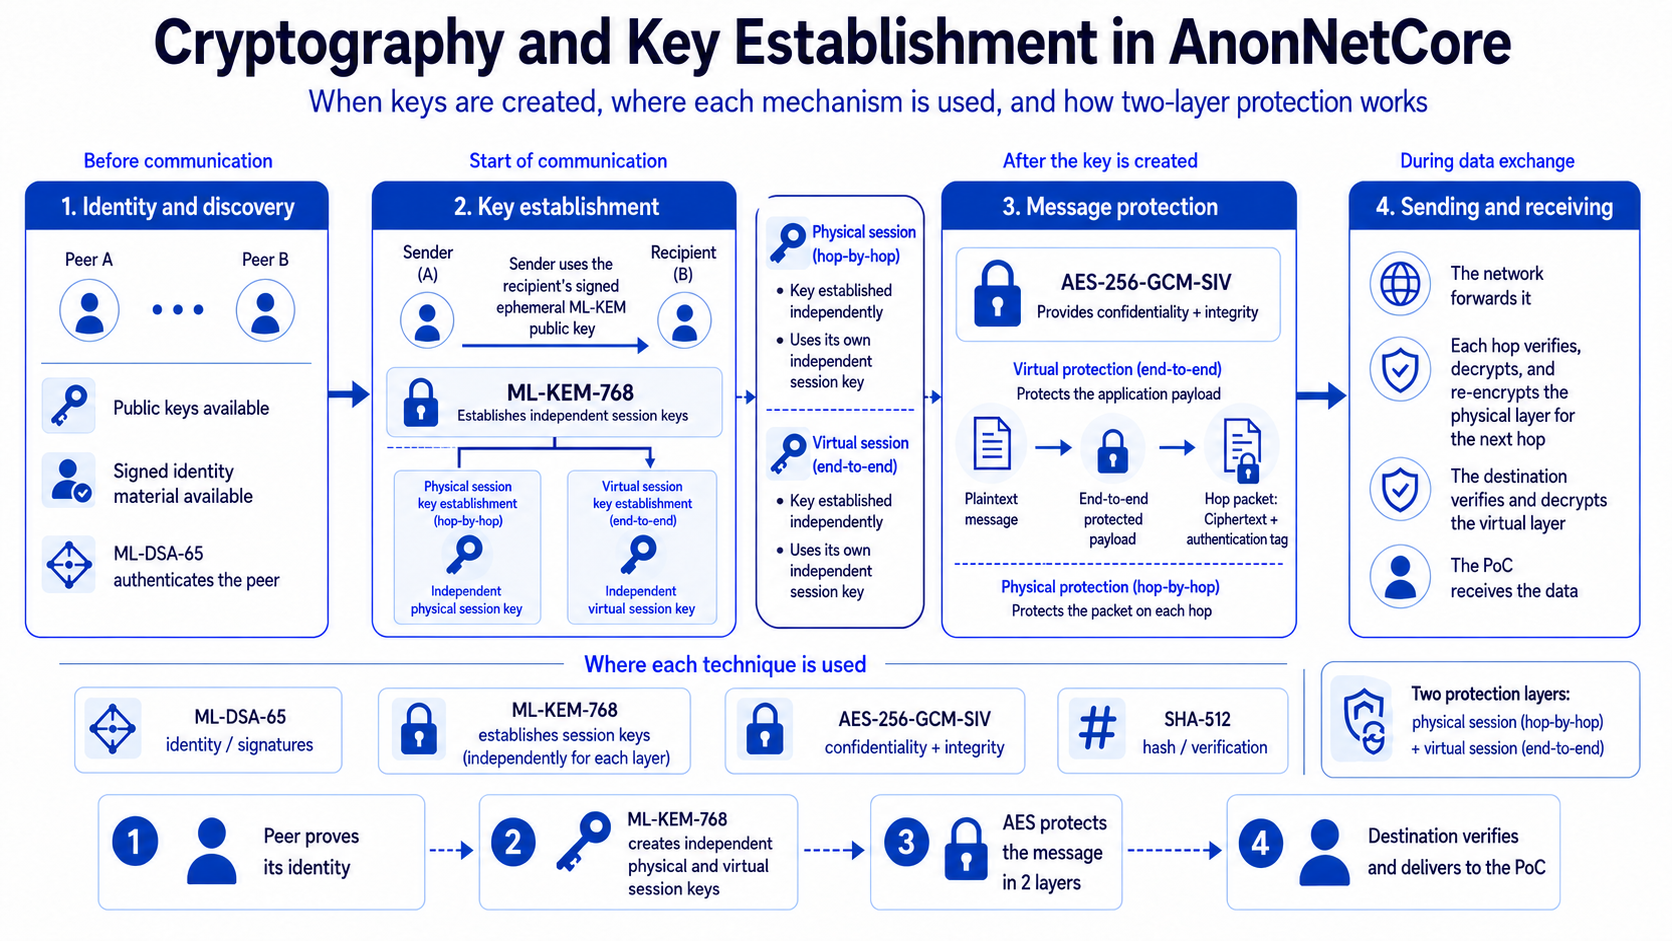
\includegraphics[width=\textwidth]{img/cryptography-key-establishment-flow.png}
\caption{Cryptographic identity, independent physical and virtual key establishment, and two-layer message protection in the implemented Core.}
\label{fig:cryptography-key-establishment-flow}
\end{figure}

The implemented virtual session message types are:

\begin{itemize}
    \item \codebreak{VIRTUAL\_\allowbreak{}SESSION\_\allowbreak{}INIT};
    \item \codebreak{VIRTUAL\_\allowbreak{}SESSION\_\allowbreak{}INIT\_\allowbreak{}OK};
    \item \codebreak{VIRTUAL\_\allowbreak{}SESSION\_\allowbreak{}KEY\_\allowbreak{}CONFIRM};
    \item \codebreak{VIRTUAL\_\allowbreak{}SESSION\_\allowbreak{}READY};
    \item \codebreak{VIRTUAL\_\allowbreak{}SESSION\_\allowbreak{}KEEPALIVE};
    \item \codebreak{VIRTUAL\_\allowbreak{}SESSION\_\allowbreak{}KEEPALIVE\_\allowbreak{}ACK};
    \item \codebreak{VIRTUAL\_\allowbreak{}SESSION\_\allowbreak{}CLOSE}.
\end{itemize}

After the session is established, application messages are sent through:

\begin{equation}
    \codemath{VIRTUAL\_\allowbreak{}SESSION\_\allowbreak{}DATA}
\end{equation}

In the social PoC, direct messages use the application message type:

\begin{equation}
    \codemath{social.direct\_\allowbreak{}message}
\end{equation}

\subsection{Reliable Session Payloads}
\label{sec:reliable-session-payloads}

The current MVP implements a lightweight reliability layer on top of active physical and virtual sessions. This mechanism is not a replacement for TCP reliability and does not attempt to solve all route-level failures. Its purpose is narrower: to provide ordered delivery, duplicate suppression, acknowledgments, and bounded retransmission for protected session payloads in a way that can also support less reliable transports in future iterations.

Reliable transmission is implemented with two envelope families:

\begin{itemize}
    \item \codebreak{PHYSICAL\_\allowbreak{}SESSION\_\allowbreak{}RELIABLE\_\allowbreak{}DATA} and \codebreak{PHYSICAL\_\allowbreak{}SESSION\_\allowbreak{}RELIABLE\_\allowbreak{}ACK} for hop-by-hop physical sessions;
    \item \codebreak{VIRTUAL\_\allowbreak{}SESSION\_\allowbreak{}RELIABLE\_\allowbreak{}DATA} and \codebreak{VIRTUAL\_\allowbreak{}SESSION\_\allowbreak{}RELIABLE\_\allowbreak{}ACK} for end-to-end virtual sessions.
\end{itemize}

Each reliable payload wraps an inner protocol message:

\begin{verbatim}
{
    "reliable_message_id": "...",
    "sequence_number": 1,
    "inner_message_type": "...",
    "inner_payload": { ... },
    "created_at": "...",
    "attempt": 1
}
\end{verbatim}

The session manager maintains in-memory reliability state per session, including the next outbound sequence number, the next expected inbound sequence number, pending outbound messages, buffered out-of-order inbound messages, and already delivered message identifiers. When a reliable payload arrives, the receiver immediately prepares an acknowledgment containing the received message identifier and sequence number. Duplicate messages are acknowledged again but not delivered twice. Out-of-order messages are buffered until the missing previous sequence numbers arrive, preserving ordered delivery to the inner protocol handler.

Retransmission is handled by \codebreak{Session\_\allowbreak{}Runtime}. The runtime periodically scans pending reliable messages and resends messages whose retry deadline has expired. Physical sessions use a fixed retry interval because they represent adjacent hop-by-hop communication. Virtual sessions use a dynamic retry interval derived from the route RTT when available, bounded by minimum and maximum configuration values. This distinction is necessary because an end-to-end virtual session may traverse a longer route than a direct physical session.

For virtual reliable payloads, an acknowledgment may also carry synchronous inner virtual responses produced while processing the delivered message. This keeps the protocol flow compact without bypassing the normal virtual-session processing path: the response is still represented as a virtual envelope and is dispatched by the virtual session handler after the reliable acknowledgment is processed.

The reliable state is runtime-only. It is not persisted as durable storage, because it represents live session delivery state and depends on active session keys, active routes, and currently reachable peers. If a session is lost, higher layers must establish a new session or retry the application-level operation.

\subsection{Protocol Message Types}
\label{sec:protocol-message-types}

Table~\ref{tab:protocol-message-types} summarizes the main implemented protocol families and message types.

{\small
\begin{longtable}{L{0.10\textwidth} L{0.19\textwidth} L{0.36\textwidth} L{0.20\textwidth}}
\caption{Implemented protocol families and message types.}
\label{tab:protocol-message-types}\\
\toprule
\textbf{Layer} & \textbf{Protocol family} & \textbf{Message types} & \textbf{Purpose} \\
\midrule
\endfirsthead

\toprule
\textbf{Layer} & \textbf{Protocol family} & \textbf{Message types} & \textbf{Purpose} \\
\midrule
\endhead

Physical & Ping &
\texttt{PING}\newline \texttt{PONG} &
Validates basic reachability and measures RTT between physical nodes. \\

Physical & Physical node info &
\codebreak{PHYSICAL\_\allowbreak{}NODE\_\allowbreak{}INFO\_\allowbreak{}REQUEST}\newline \codebreak{PHYSICAL\_\allowbreak{}NODE\_\allowbreak{}INFO\_\allowbreak{}RESPONSE} &
Obtains identity and advertised endpoints of physical nodes. \\

Physical & Peer exchange &
\codebreak{PHYSICAL\_\allowbreak{}NODE\_\allowbreak{}INFO\_\allowbreak{}EXCHANGE\_\allowbreak{}REQUEST}\newline \codebreak{PHYSICAL\_\allowbreak{}NODE\_\allowbreak{}INFO\_\allowbreak{}EXCHANGE\_\allowbreak{}RESPONSE}\newline \codebreak{PHYSICAL\_\allowbreak{}NODE\_\allowbreak{}INFO\_\allowbreak{}ANNOUNCE} &
Spreads known physical nodes beyond the initial bootstrap list. \\

Physical & Physical session &
\codebreak{PHYSICAL\_\allowbreak{}SESSION\_\allowbreak{}INIT}\newline \codebreak{PHYSICAL\_\allowbreak{}SESSION\_\allowbreak{}INIT\_\allowbreak{}OK}\newline \codebreak{PHYSICAL\_\allowbreak{}SESSION\_\allowbreak{}KEY\_\allowbreak{}CONFIRM}\newline \codebreak{PHYSICAL\_\allowbreak{}SESSION\_\allowbreak{}READY}\newline \codebreak{PHYSICAL\_\allowbreak{}SESSION\_\allowbreak{}KEEPALIVE}\newline \codebreak{PHYSICAL\_\allowbreak{}SESSION\_\allowbreak{}KEEPALIVE\_\allowbreak{}ACK}\newline \codebreak{PHYSICAL\_\allowbreak{}SESSION\_\allowbreak{}CLOSE} &
Creates and maintains secure hop-by-hop sessions between adjacent physical nodes. \\

Physical & Physical reliable session &
\codebreak{PHYSICAL\_\allowbreak{}SESSION\_\allowbreak{}RELIABLE\_\allowbreak{}DATA}\newline \codebreak{PHYSICAL\_\allowbreak{}SESSION\_\allowbreak{}RELIABLE\_\allowbreak{}ACK} &
Wraps physical-session payloads with sequence numbers, acknowledgments, duplicate suppression, ordered delivery, and bounded retransmission. \\

Physical & Physical relay &
\codebreak{PHYSICAL\_\allowbreak{}RELAY\_\allowbreak{}DATA} &
Encapsulates a physical packet through a relay-capable public physical node using active physical sessions with the sender and target. \\

Physical & DHT &
\codebreak{DHT\_\allowbreak{}PUBLISH}\newline \codebreak{DHT\_\allowbreak{}QUERY}\newline \codebreak{DHT\_\allowbreak{}RESULT} &
Publishes and retrieves distributed records across DPNT, DRT, DDT, DPT, and DTT namespaces. \\

Physical & Route build &
\codebreak{ROUTE\_\allowbreak{}CREATE}\newline \codebreak{ROUTE\_\allowbreak{}CREATE\_\allowbreak{}KEM\_\allowbreak{}INFO}\newline \codebreak{ROUTE\_\allowbreak{}CREATE\_\allowbreak{}VALIDATE\_\allowbreak{}AND\_\allowbreak{}PUBLISH}\newline \codebreak{ROUTE\_\allowbreak{}CREATE\_\allowbreak{}PING}\newline \codebreak{ROUTE\_\allowbreak{}CREATE\_\allowbreak{}PONG}\newline \codebreak{ROUTE\_\allowbreak{}CREATE\_\allowbreak{}OK}\newline \codebreak{ROUTE\_\allowbreak{}CREATE\_\allowbreak{}FAIL} &
Creates physical routes that allow virtual nodes to publish entry points in the DRT. \\

Physical & Route execute &
\codebreak{ROUTE\_\allowbreak{}DATA} &
Carries virtual envelopes through already created physical routes. \\

Virtual & Virtual session &
\codebreak{VIRTUAL\_\allowbreak{}SESSION\_\allowbreak{}INIT}\newline \codebreak{VIRTUAL\_\allowbreak{}SESSION\_\allowbreak{}INIT\_\allowbreak{}OK}\newline \codebreak{VIRTUAL\_\allowbreak{}SESSION\_\allowbreak{}KEY\_\allowbreak{}CONFIRM}\newline \codebreak{VIRTUAL\_\allowbreak{}SESSION\_\allowbreak{}READY}\newline \codebreak{VIRTUAL\_\allowbreak{}SESSION\_\allowbreak{}KEEPALIVE}\newline \codebreak{VIRTUAL\_\allowbreak{}SESSION\_\allowbreak{}KEEPALIVE\_\allowbreak{}ACK}\newline \codebreak{VIRTUAL\_\allowbreak{}SESSION\_\allowbreak{}CLOSE} &
Establishes and maintains end-to-end sessions between virtual nodes. \\

Virtual & Virtual reliable session &
\codebreak{VIRTUAL\_\allowbreak{}SESSION\_\allowbreak{}RELIABLE\_\allowbreak{}DATA}\newline \codebreak{VIRTUAL\_\allowbreak{}SESSION\_\allowbreak{}RELIABLE\_\allowbreak{}ACK} &
Wraps virtual-session payloads with ordered delivery, acknowledgments, retransmission, and optional synchronous inner virtual responses carried by acknowledgments. \\

Virtual & Virtual message &
\codebreak{VIRTUAL\_\allowbreak{}SESSION\_\allowbreak{}DATA} &
Transports application-level messages over an active virtual session. \\

Virtual & Virtual content &
\codebreak{VIRTUAL\_\allowbreak{}CONTENT\_\allowbreak{}INFO\_\allowbreak{}REQUEST}\newline \codebreak{VIRTUAL\_\allowbreak{}CONTENT\_\allowbreak{}INFO\_\allowbreak{}RESPONSE}\newline \codebreak{VIRTUAL\_\allowbreak{}CONTENT\_\allowbreak{}RANGE\_\allowbreak{}REQUEST}\newline \codebreak{VIRTUAL\_\allowbreak{}CONTENT\_\allowbreak{}RANGE\_\allowbreak{}RESPONSE}\newline \codebreak{VIRTUAL\_\allowbreak{}CONTENT\_\allowbreak{}NOT\_\allowbreak{}FOUND}\newline \codebreak{VIRTUAL\_\allowbreak{}CONTENT\_\allowbreak{}RANGE\_\allowbreak{}DENIED}\newline \codebreak{VIRTUAL\_\allowbreak{}CONTENT\_\allowbreak{}RANGE\_\allowbreak{}ERROR} &
Retrieves content metadata and byte ranges from virtual content holders. \\
\bottomrule
\end{longtable}
}

\subsection{Local Persistence Model}
\label{sec:local-persistence-model}

Local persistence is implemented with SQLite through SQLAlchemy. Persistent state includes identities, endpoints, DHT records, route metadata, content metadata, and operational logs. Runtime-only state such as active sockets, handshake state, cryptographic session secrets, temporary buffers, and reliable-session delivery windows remains in memory.

The main persistence rule is that stable identifiers and metadata are persisted, while active cryptographic material, live network resources, pending reliable acknowledgments, in-flight retransmission state, and ordered-delivery buffers are not persisted without protection.

Table~\ref{tab:persistence-summary} summarizes the main persistence entities.

\begin{table}[H]
\centering
\caption{Summary of local persistence entities.}
\label{tab:persistence-summary}
\begin{tabularx}{\textwidth}{L{0.27\textwidth} Y}
\toprule
\textbf{Entity} & \textbf{Purpose} \\
\midrule
\codebreak{local\_\allowbreak{}physical\_\allowbreak{}node\_\allowbreak{}identity} & Stores the local physical node identity and key material. \\
\codebreak{local\_\allowbreak{}virtual\_\allowbreak{}node\_\allowbreak{}identity} & Stores virtual identities hosted by the local physical node. \\
\codebreak{remote\_\allowbreak{}physical\_\allowbreak{}node\_\allowbreak{}identity} & Caches known remote physical nodes and operational metadata. \\
\codebreak{node\_\allowbreak{}endpoint} & Stores advertised endpoints for known physical nodes. \\
\codebreak{remote\_\allowbreak{}virtual\_\allowbreak{}node\_\allowbreak{}identity} & Caches known remote virtual nodes. \\
\codebreak{dht\_\allowbreak{}record} & Stores local replicas of distributed records from DPNT, DRT, DDT, DPT, and DTT. \\
\codebreak{route\_\allowbreak{}resolution} & Stores local route mappings required by initiators, hops, and final endpoints. \\
\codebreak{content\_\allowbreak{}object} & Stores metadata for locally persisted content objects. \\
\codebreak{content\_\allowbreak{}advertisement} & Tracks content announcements published by local virtual nodes in the DDT. \\
\codebreak{seen\_\allowbreak{}hash} & Avoids repeated processing of already seen packets, messages, or objects. \\
\codebreak{local\_\allowbreak{}event\_\allowbreak{}log} & Stores operational events for debug and audit support. \\
\bottomrule
\end{tabularx}
\end{table}

This model supports the core requirement of the architecture: distributed references use compact hash-based identifiers, while complete public keys remain available when signatures or identity reconstruction are required.

\subsection{Local API}
\label{sec:local-api-implementation}

The local API exposes core functionality to external applications. The API is local by default and is intended to be consumed by desktop applications, local HTML interfaces, scripts, and integration tests.

The HTTP API is exposed at:

\begin{equation}
    \codemath{http:\allowbreak{}/\allowbreak{}/\allowbreak{}127.0.0.1:\allowbreak{}18080}
\end{equation}

The WebSocket event stream is exposed at:

\begin{equation}
    \codemath{ws:\allowbreak{}/\allowbreak{}/\allowbreak{}127.0.0.1:\allowbreak{}18081/\allowbreak{}v1/\allowbreak{}events}
\end{equation}

The API includes endpoints for health checks, debug snapshots, virtual node management, virtual signatures, DHT publish/query operations, virtual sessions, virtual messages, content storage, content downloads, and event subscriptions. Long operations, such as DHT publication from the user interface, can be executed through asynchronous jobs.

Table~\ref{tab:api-summary} summarizes the main API groups.

\begin{table}[H]
\centering
\caption{Summary of implemented local API groups.}
\label{tab:api-summary}
\begin{tabularx}{\textwidth}{L{0.24\textwidth} Y}
\toprule
\textbf{API group} & \textbf{Purpose} \\
\midrule
Status and debug & Provides \texttt{/health}, \texttt{/v1/status}, and \texttt{/debug/state}. \\
Virtual nodes & Creates and lists local VNs and registers known remote VNs. \\
Virtual signatures & Allows applications to sign payloads with local VN keys and verify VN signatures. \\
DHT & Computes DHT keys, publishes records, queries records, and manages publish jobs. \\
Virtual sessions & Opens, lists, sends messages through, and closes virtual sessions. \\
Virtual messages & Subscribes to application message types and reads received messages. \\
Content & Stores local content, retrieves metadata, reads byte ranges, and publishes DDT holders. \\
Downloads & Starts and tracks virtual content downloads. \\
WebSocket events & Emits events such as received virtual messages and content publication updates. \\
\bottomrule
\end{tabularx}
\end{table}

The API does not replace the internal protocols. Instead, it calls the corresponding services and protocol clients inside the core. This design allows external applications to use the network without depending on internal Python modules.

From the application's perspective, this boundary turns distributed networking operations into a small local service interface. Profile publication invokes content storage followed by DDT and DPT publication; feed reconstruction invokes DPT resolution, DDT holder discovery, and content download; direct messaging invokes DRT resolution and virtual-session establishment; and WebSocket events deliver incoming messages without requiring the browser to poll protocol state. The application therefore benefits from peer discovery, route construction, persistence, cryptographic sessions, and transport heterogeneity while remaining independent of their internal implementations.

Figure~\ref{fig:poc-core-overlay-integration} provides a didactic view of this boundary. An external application submits a request through the local HTTP API, receives asynchronous events through WebSocket, and delegates identity protection, route resolution, session establishment, persistence, and forwarding to the Core. The destination Core reverses the layered processing and delivers the resulting application event locally, while intermediate physical peers process only the forwarding and hop-protection information required at their respective positions.

\begin{figure}[H]
\centering
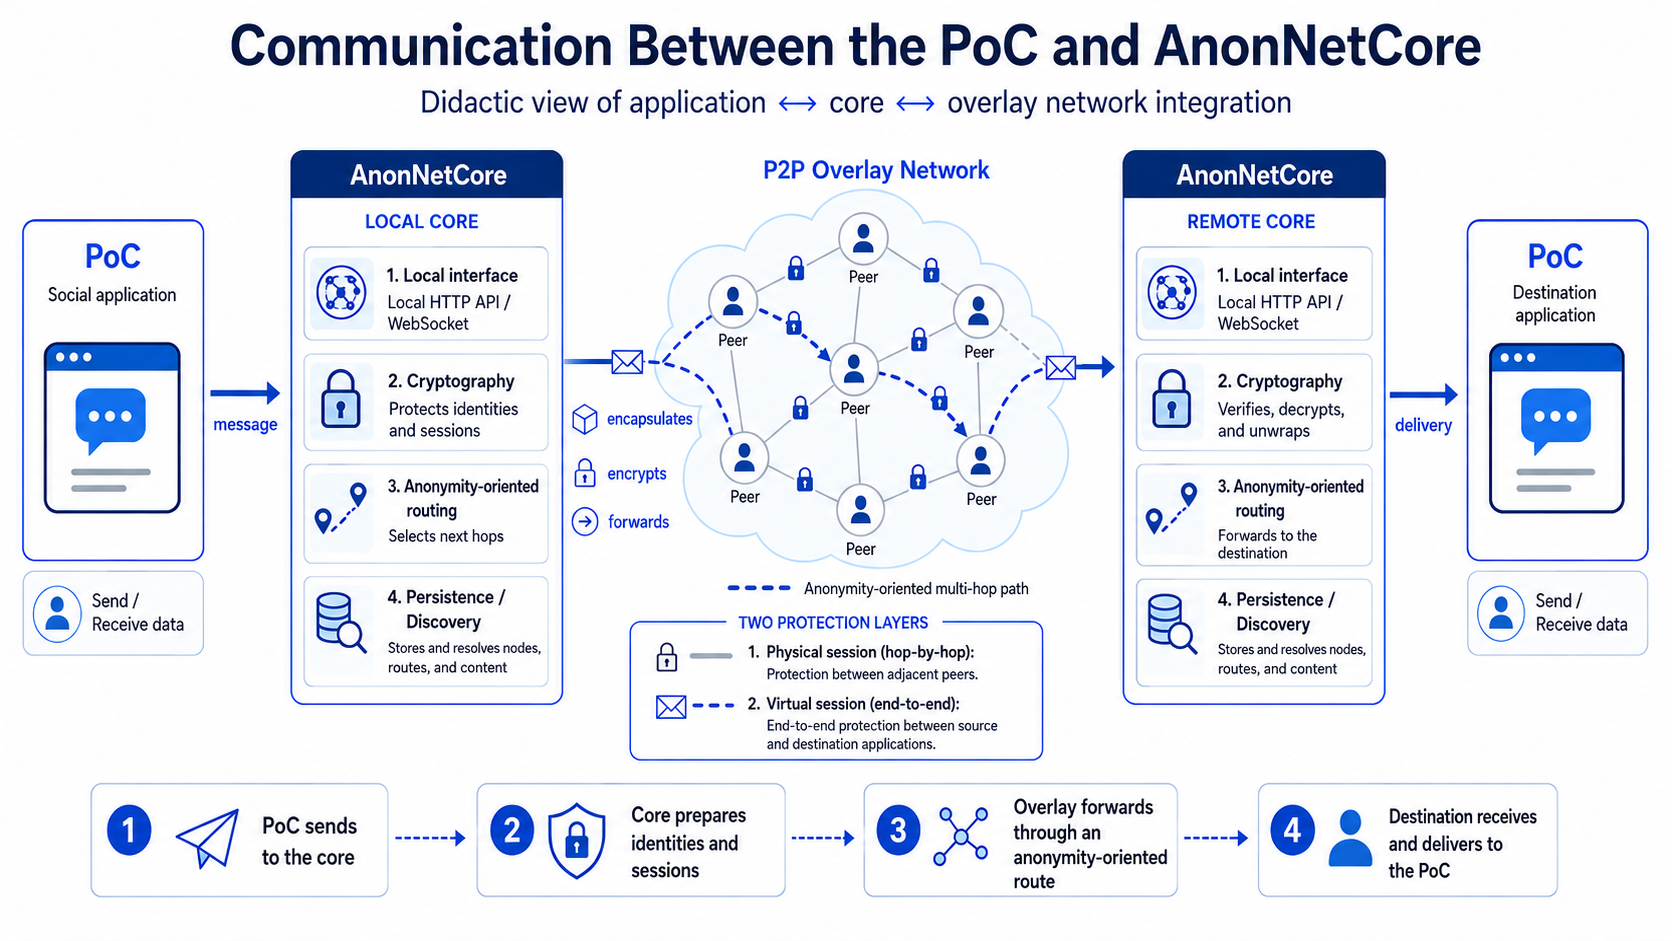
\includegraphics[width=\textwidth]{img/poc-core-overlay-integration.png}
\caption{Integration flow between the social PoC, the local Core, the physical overlay route, and the destination application.}
\label{fig:poc-core-overlay-integration}
\end{figure}

\subsection{Social Proof of Concept}
\label{sec:social-poc-implementation}

A social proof of concept was implemented to validate the architecture from the perspective of an external application. The PoC is a local HTML/JavaScript interface that communicates with the core through the local API.

The social model is intentionally simple: in the social PoC, one virtual node corresponds to one social profile.

A profile state contains name, biography, profile photo, friend list, posts, and local metadata. The current profile state is stored as a local content object. The virtual node then publishes itself as a holder of that content in the DDT and updates a DPT pointer to reference the most recent state object.

The DPT logical key used by the PoC is:

\begin{equation}
    \texttt{logical\_key} = \texttt{virtual\_node\_id|profile}
\end{equation}

The physical DHT key is derived from this logical key:

\begin{equation}
    \texttt{dpt\_key} = SHA512(\texttt{dpt|virtual\_node\_id|profile})
\end{equation}

The DPT record contains:

\begin{equation}
    \texttt{target\_ref} = \texttt{content\_id}
\end{equation}

Since the DPT is signed by the owner virtual node, other peers can verify that the pointer belongs to the claimed profile. During validation, peers compute \codebreak{SHA\allowbreak{}512(pk\_\allowbreak{}virtual\_\allowbreak{}node\_\allowbreak{}owner)} and confirm that it matches the \texttt{virtual\_node\_id} used in the DPT key. To read a friend's profile, the application queries the friend's DPT, validates the pointer, resolves the referenced content in the DDT, downloads the content from a holder, and renders the posts in the feed.

Direct messages use virtual sessions. The application requests a session with a friend virtual node, the core resolves the friend's DRT entry, resolves the entry point in the DPNT, establishes the virtual session through \codebreak{ROUTE\_\allowbreak{}DATA}, and sends the message using \codebreak{VIRTUAL\_\allowbreak{}SESSION\_\allowbreak{}DATA} with the application type \codebreak{social.direct\_\allowbreak{}message}.

\subsection{Experimental Execution}
\label{sec:experimental-execution}

The implementation includes three main execution scripts: one to run a local core, one to run the social PoC with cluster and Debug Console support, and one to run the official integration smokes. The following commands are representative examples:

\begin{verbatim}
.\.venv\Scripts\python.exe scripts\run_core.py

.\.venv\Scripts\python.exe scripts\run_poc.py 10

.\.venv\Scripts\python.exe scripts\run_smokes.py 10
\end{verbatim}

The experimental environment validates execution with multiple local or containerized nodes. The Debug Console and the \texttt{/debug/state} endpoint were used to inspect peers, sessions, DHT records, route state, runtime status, and potential operational inconsistencies.

\subsection{Validation and Test Results}
\label{sec:validation-test-results}

The MVP was validated through smoke tests and the social PoC. The tests are flow-oriented: instead of only testing isolated functions, they instantiate real cores and exercise protocol interactions across the implemented layers.

Table~\ref{tab:smoke-tests} summarizes the main validation tests.

\begin{table}[H]
\centering
\caption{Implemented smoke tests and validation goals.}
\label{tab:smoke-tests}
\setlength{\tabcolsep}{4pt}
\begin{tabularx}{\textwidth}{C{0.08\textwidth} L{0.29\textwidth} Y}
\toprule
\textbf{Status} & \textbf{Test} & \textbf{Validation goal} \\
\midrule
\statusvalidated & \codebreak{core\_\allowbreak{}full\_\allowbreak{}flow\_\allowbreak{}smoke.\allowbreak{}py} & Validates the core as an integrated system, including Docker cluster startup, randomized transport topology, bootstrap, physical peer validation, DHT publish/query, route maintenance, DRT resolution, virtual sessions, virtual messages, content transfer, local API access, WebSocket events, reliable delivery, and debug-state inspection. \\
\statusvalidated & \codebreak{poc\_\allowbreak{}full\_\allowbreak{}flow\_\allowbreak{}smoke.\allowbreak{}py} & Validates the external social PoC through the public local API, including creation of two virtual-node profiles, DPT/DDT publication, friendship, remote profile resolution, feed construction from a friend's posts, direct messages, and browser-facing JavaScript service behavior. \\
\statusvalidated & \codebreak{scripts/\allowbreak{}run\_\allowbreak{}smokes.\allowbreak{}py} & Orchestrates the official smoke suite, resets local cluster data, starts the requested number of nodes, prints the randomized topology, runs the core and PoC flows in order, reports pass/fail status, and stops the cluster after execution. \\
\bottomrule
\end{tabularx}
\end{table}

Table~\ref{tab:experimental-results-summary} summarizes the functional outcomes observed during validation.

\begin{table}[H]
\centering
\caption{Summary of experimental validation results.}
\label{tab:experimental-results-summary}
\begin{tabularx}{\textwidth}{L{0.32\textwidth} L{0.20\textwidth} Y}
\toprule
\textbf{Experiment} & \textbf{Observed result} & \textbf{Interpretation} \\
\midrule
Local physical cluster execution & \statusvalidated & Multiple physical nodes were instantiated and connected through the bootstrap process. \\
Virtual node creation & \statusvalidated & The core was able to create and maintain independent virtual identities. \\
DRT route publication & \statusvalidated & Virtual node reachability information was published and resolved through DHT records. \\
Virtual session establishment & \statusvalidated & Virtual endpoints established sessions over physical route structures. \\
Virtual message delivery & \statusvalidated & Application messages were delivered through the virtual session pipeline. \\
Content advertisement and retrieval & \statusvalidated & Content objects were stored, advertised in the DDT, resolved, and downloaded using byte ranges. \\
Social PoC integration & \statusvalidated & The external application consumed the local API to create profiles, posts, friendships, feed entries, and direct messages. \\
\bottomrule
\end{tabularx}
\end{table}

Together, the results cover the complete prototype path: cluster bootstrap and physical validation; virtual identity and route maintenance; DRT/DPNT resolution; virtual sessions and messages; byte-range content publication and retrieval; external PoC access through the local API; and runtime inspection of peers, sessions, DHT records, routes, and warnings. Figures~\ref{fig:cluster-log}, \ref{fig:poc-social-profile}, \ref{fig:debug-console-overview}, and \ref{fig:smokes-passing} retain one representative artifact for each validation surface. The complete screenshot set remains available in the repository under \texttt{thesis/assets/img}.

\begin{figure}[H]
\centering
\IfFileExists{assets/img/cluster-console-1.png}{
    \thesisfiguregraphic{assets/img/cluster-console-1.png}
}{
    \fbox{
        \parbox{0.9\textwidth}{
            \centering
            Placeholder: cluster execution console showing multiple physical nodes and randomized transport profiles.
        }
    }
}
\caption{Cluster execution console showing multiple physical nodes running in the experimental Docker environment.}
\label{fig:cluster-log}
\end{figure}

\begin{figure}[H]
\centering
\IfFileExists{assets/img/poc-1.png}{
    \thesisfiguregraphic{assets/img/poc-1.png}
}{
    \fbox{
        \parbox{0.9\textwidth}{
            \centering
            Placeholder: social PoC interface showing profile state, friends, and feed.
        }
    }
}
\caption{Social proof of concept showing profile state, friends, and feed synchronization through the local API.}
\label{fig:poc-social-profile}
\end{figure}

\begin{figure}[H]
\centering
\IfFileExists{assets/img/debug-console-1.png}{
    \thesisfiguregraphic{assets/img/debug-console-1.png}
}{
    \fbox{
        \parbox{0.9\textwidth}{
            \centering
            Placeholder: Debug Console overview.
        }
    }
}
\caption{Debug Console overview used to observe the experimental execution.}
\label{fig:debug-console-overview}
\end{figure}

\begin{figure}[H]
\centering
\IfFileExists{assets/img/smoke-console-7.png}{
    \thesisfiguregraphic{assets/img/smoke-console-7.png}
}{
    \fbox{
        \parbox{0.9\textwidth}{
            \centering
            Placeholder: terminal output showing final smoke pass/fail summary.
        }
    }
}
\caption{Final smoke-test summary showing the successful integrated Core and social PoC validation flows.}
\label{fig:smokes-passing}
\end{figure}

\subsection{Comparison with Related Systems and Concepts}
\label{sec:implementation-comparison}

The implementation is not intended to reproduce an existing system directly. Instead, it combines concepts from structured DHTs, peer-to-peer overlays, anonymous routing, and post-quantum cryptography into a prototype tailored to the proposed architecture.

Table~\ref{tab:comparison-related-work} summarizes the main comparisons.

\begingroup
\small
\renewcommand{\arraystretch}{1.05}
\begin{longtable}{L{0.20\textwidth} L{0.34\textwidth} L{0.34\textwidth}}
\caption{Comparison between the implemented MVP and related systems or concepts.}
\label{tab:comparison-related-work}\\
\toprule
\textbf{Reference concept} & \textbf{Similarity} & \textbf{Difference in the MVP} \\
\midrule
\endfirsthead
\caption[]{Comparison between the implemented MVP and related systems or concepts (continued).}\\
\toprule
\textbf{Reference concept} & \textbf{Similarity} & \textbf{Difference in the MVP} \\
\midrule
\endhead
\midrule
\multicolumn{3}{r}{\footnotesize Continued on next page.}\\
\endfoot
\bottomrule
\endlastfoot
Kademlia / DHTs~[2] &
The MVP uses hash-based keys, XOR distance, and responsibility by proximity. &
The implementation does not yet implement a complete Kademlia routing table, iterative lookup procedure, bucket management, or mature churn handling. \\

Peer-to-peer overlay networks~[1], [2], [3] &
The architecture separates logical overlay behavior from physical network connections and allows nodes to exchange resources without a central application server. &
The prototype currently runs in controlled local or Docker environments and still requires future work for Internet-scale churn, NAT traversal, and large-scale peer discovery. \\

Tor / onion routing~[20] &
The route layer also separates intermediate forwarding from final virtual semantics, and intermediate hops do not need to know the complete route. &
The MVP does not implement Tor's complete onion routing design, directory authority model, circuit construction protocol, relay ecosystem, or mature resistance against global traffic correlation. \\

I2P / garlic routing~[21] &
The architecture shares the goal of hiding communication relationships through indirect overlay routing and separation between network-level and application-level identities. &
The MVP does not implement I2P's garlic routing model, tunnel management, network database, lease sets, or mature anonymity mechanisms, focusing instead on validating virtual identities, DHT-based discovery, and route construction in a simplified prototype. \\

Content-addressed systems~[19] &
Content is addressed by hash and announced through distributed references. &
The MVP separates pointer resolution, holder discovery, and virtual content transfer through DPT, DDT, and virtual sessions rather than reproducing IPFS directly. \\

Post-quantum cryptography~[13], [14], [26] &
The implementation uses post-quantum KEM and signature algorithms when available, combined with symmetric encryption for session payloads. &
The prototype has not undergone formal cryptographic audit, side-channel analysis, or production hardening of key storage and cryptographic lifecycle management. \\
\end{longtable}
\endgroup

The main contribution of the implementation is the integration of these ideas into a layered architecture in which physical nodes, virtual identities, DHT records, route entries, sessions, and application objects are explicitly separated.

\subsection{Known Limitations and Future Work}
\label{sec:implementation-limitations-future-work}

The MVP validates the core architecture, but several components require further development before the system can be considered robust in public networks. Table~\ref{tab:limitations-future-work} summarizes the main limitations and future work.

\begingroup
\small
\renewcommand{\arraystretch}{1.08}
\begin{longtable}{L{0.19\textwidth} L{0.34\textwidth} L{0.35\textwidth}}
\caption{Current limitations and future work.}
\label{tab:limitations-future-work}\\
\toprule
\textbf{Area} & \textbf{Current limitation} & \textbf{Future work} \\
\midrule
\endfirsthead
\caption[]{Current limitations and future work (continued).}\\
\toprule
\textbf{Area} & \textbf{Current limitation} & \textbf{Future work} \\
\midrule
\endhead
\midrule
\multicolumn{3}{r}{\footnotesize Continued on next page.}\\
\endfoot
\bottomrule
\endlastfoot
NAT traversal & The MVP includes TCP, experimental UDP transport, and relay-assisted physical forwarding, but it does not implement complete NAT traversal. & Implement UDP hole punching, STUN/TURN support, relay hardening, and later QUIC-based transport. \\

DHT routing & The DHT uses XOR proximity and replication but does not yet include a complete Kademlia-style routing table. & Implement buckets, iterative lookup, routing table refresh, churn handling, and more complete proximity search. \\

Anti-abuse & The MVP includes lightweight DHT publication proof-of-work, but there is no mature defense against Sybil attacks, flooding, spam, or coordinated malicious peers. & Add adaptive proof-of-work, peer scoring, rate limits per peer and namespace, invalid signature penalties, and origin concentration detection. \\

Scalability & Tests currently focus on local processes and Docker clusters. & Execute long-running experiments with larger clusters, churn, latency, packet loss, and heterogeneous nodes. \\

Security hardening & The MVP has not undergone formal security audit and local private key protection still requires strengthening. & Harden key storage, review cryptographic lifecycles, add secure local access control, and perform external audits. \\

Route privacy & The route mechanism reduces local knowledge at each hop, but does not provide full protection against global correlation. & Study stronger onion-like encapsulation, cover traffic, route rotation, and traffic analysis resistance. \\

Reliability & The MVP implements basic reliable session payloads with sequence numbers, acknowledgments, duplicate detection, ordered delivery, and retransmission, but it does not yet include advanced transport behavior. & Add congestion control, adaptive backoff, route failover, session migration policies, and broader reliability coverage for additional control protocols. \\

DTT and large lists & The DTT is modeled but not central to the current PoC, and large DDT/DTT lists are not sharded. & Implement sharding, pagination, tag indexing, expiration policies, and garbage collection for large distributed records. \\

Application PoC & The social PoC stores profile photos as data URLs and downloads complete friend states. & Store media as separate content objects, add pagination, access control, privacy settings, moderation, and efficient feed synchronization. \\
\end{longtable}
\endgroup

These limitations do not invalidate the MVP. Instead, they define the boundary between an experimental prototype and a production-grade decentralized network.

\subsection{Chapter Summary}
\label{sec:implementation-summary}

This chapter presented the implementation of the proposed architecture as a functional experimental MVP. The prototype implements a physical layer, virtual layer, TCP transport, experimental UDP transport, relay-assisted physical forwarding, DHT namespaces, route construction, route execution, reliable physical and virtual session payloads, content transfer, local HTTP/WebSocket API, and a social proof of concept.

The implementation demonstrates that the proposed separation between physical nodes and virtual nodes is feasible, that distributed records can be used to locate physical nodes, virtual routes, content holders, and mutable pointers, and that an external application can use the network through a local API. The smoke tests and social PoC validate the main protocol flows expected from the architecture, including route maintenance, DHT publication proof-of-work, route-based virtual sessions, direct messages, content download by byte ranges, and runtime observability.

At the same time, the implementation remains intentionally limited. It is a research prototype designed to validate architecture and integration, not a hardened public network. Future work should focus on complete NAT traversal, relay hardening, complete Kademlia-style routing, stronger anti-abuse mechanisms, scalability tests, reliability under churn and packet loss, cryptographic hardening, formal auditing, and more realistic application-level privacy controls.

















\section{Conclusion}
\label{sec:conclusion}

This work presented the design, implementation, and experimental validation of a decentralized peer-to-peer overlay network architecture focused on secure communication, data persistence, and support for decentralized applications. The proposed architecture was motivated by the limitations of centralized communication models, the increasing relevance of privacy-preserving systems, and the need to investigate network designs that combine peer-to-peer communication, distributed discovery, content-addressed storage, routing abstraction, and post-quantum cryptographic mechanisms.

The main objective of the project was achieved through the development of the \textit{AnonNetCore Python MVP}, an experimental prototype that implements the core concepts proposed throughout this work. The implemented system separates physical nodes, which represent real network processes, from virtual nodes, which represent logical overlay identities. This separation allowed the architecture to decouple transport-level connectivity from application-level identity, enabling multiple virtual identities to coexist over the same physical node and allowing applications to interact with the network through a higher-level abstraction.

The implementation also demonstrated that distributed tables can be used as a common foundation for multiple discovery and persistence functions. The DPNT was used to describe and locate physical nodes; the DRT was used to publish entry points for virtual nodes; the DDT was used to announce content holders; and the DPT was used to maintain mutable signed references to application state. Together, these structures provided a practical mechanism for peer discovery, route resolution, content lookup, and application-level state publication. The MVP also introduced lightweight publication proof-of-work for DHT payloads, adding an explicit computational cost to distributed writes while preserving cheap verification by responsible peers.

Another important result was the implementation of route creation and route execution mechanisms. The prototype showed that virtual communication can be transported through physical routes using path identifiers and encapsulated virtual envelopes. In this model, intermediate physical nodes only need to process local forwarding information, while virtual sessions remain logically end-to-end between virtual identities. This validates the feasibility of the proposed separation between the physical routing layer and the virtual communication layer.

The physical communication layer also advanced beyond the original TCP-only validation path. The MVP includes TCP transport, experimental UDP transport with compact binary fragmentation, and relay-assisted TCP forwarding for private physical nodes. These mechanisms are still experimental, but they validate the modular transport abstraction expected by the architecture and show that direct and relay-assisted communication can be handled without changing the higher-level virtual-session model.

The security and delivery mechanisms were also partially validated. The prototype uses post-quantum key-establishment and signature primitives when available, AES-256-GCM-SIV authenticated encryption, associated authenticated data for selected public metadata, and reliable session payloads with sequence numbers, acknowledgments, duplicate detection, ordered delivery, and bounded retransmission. These mechanisms do not make the prototype production-ready, but they demonstrate that the architecture can combine hop-by-hop protection, end-to-end virtual sessions, and practical delivery controls in a single protocol stack.

The local API and the social proof of concept further demonstrated that the implemented core can be consumed by external applications without requiring direct access to internal protocol modules. The social PoC used virtual nodes as profiles, DPT records as mutable profile pointers, DDT records for content holder discovery, DRT records for virtual node reachability, and virtual sessions for direct messages. This integration provided evidence that the proposed architecture can support decentralized application workflows beyond isolated protocol tests.

The experimental validation was performed through smoke tests, integration scripts, local clusters, debug snapshots, and the social proof of concept. These tests exercised the main protocol flows of the MVP, including bootstrap, peer validation, heterogeneous transport execution, DHT publication and query, route maintenance, virtual session establishment, reliable virtual message delivery, content transfer by byte ranges, HTTP/WebSocket API usage, and social profile synchronization. Therefore, although the prototype was evaluated in a controlled environment, it successfully demonstrated the functional viability of the proposed architecture.

However, the implementation must be understood as an experimental MVP rather than a production-ready network. Several limitations remain. The current prototype does not yet implement complete NAT traversal, QUIC transport, mature relay infrastructure, full Kademlia-style routing tables, robust anti-abuse mechanisms, Sybil resistance, reputation systems, large-scale churn handling, formal cryptographic auditing, or complete protection against global traffic correlation. These limitations are expected for a research prototype and define the boundary between the validated architectural model and a deployable public network.

Even with these limitations, the project contributes a concrete and extensible architecture for decentralized overlay networks. Its main contribution is not only the implementation of individual mechanisms, but the integration of physical nodes, virtual nodes, transport adapters, relay forwarding, distributed tables, proof-of-work-protected DHT writes, route construction, virtual sessions, reliable payload delivery, content transfer, local APIs, WebSocket events, observability tools, and an application-level proof of concept into a single coherent experimental system. This integration demonstrates that the proposed model can serve as a foundation for future research and development in secure decentralized applications.

Future work should focus on hardening the prototype and extending it toward real-world deployment conditions. The most relevant directions include implementing UDP hole punching, hardening relay fallback, adding QUIC support, replacing the simplified DHT behavior with a complete Kademlia-like routing layer, evolving publication proof-of-work and peer scoring, improving protection against Sybil and flooding attacks, executing larger-scale experiments with churn and packet loss, strengthening local key protection, separating media objects from social profile state, and performing a formal security review.

In conclusion, this work showed that it is feasible to design and implement a modular decentralized overlay architecture that supports secure communication, distributed discovery, persistent content references, virtual identities, and decentralized application integration. The resulting MVP validates the core architectural hypothesis of the project and establishes a practical foundation for future iterations aimed at scalability, robustness, stronger anonymity, and production-grade security.






\section*{Declaration of Artificial Intelligence Use}

Artificial Intelligence tools were used as auxiliary support during the development
of this work, exclusively to assist with the revision, organization, standardization,
and formal improvement of texts, code fragments, technical documentation, and
\LaTeX{} structures.

The purpose of using these tools was to improve clarity, cohesion, formatting,
technical terminology, and academic style. These tools were not used to replace the
intellectual authorship of the work, define the results, conduct the research, create
the scientific proposal, or generate technical content without validation by the
author.

All conceptual, architectural, methodological, and technical decisions presented in
this work were defined, reviewed, and validated by the author. The final content,
including explanations, models, design choices, code, analyses, and conclusions,
remains the full responsibility of the author.





\section*{References}
\begingroup
\setlength{\leftskip}{0.5cm}
\setlength{\parindent}{-0.5cm}
\setlength{\parskip}{6pt}

[1] STOICA, Ion; MORRIS, Robert; KARGER, David; KAASHOEK, M. Frans; BALAKRISHNAN, Hari (2001). 
\textit{Chord: A Scalable Peer-to-Peer Lookup Protocol for Internet Applications}. 
In: \textit{Proceedings of the ACM SIGCOMM 2001 Conference}. 
New York: ACM, 2001. p. 149--160.

[2] MAYMOUNKOV, Petar; MAZIERES, David (2002). 
\textit{Kademlia: A Peer-to-Peer Information System Based on the XOR Metric}. 
In: \textit{Proceedings of the 1st International Workshop on Peer-to-Peer Systems (IPTPS)}. 
Berlin: Springer, 2002. p. 53--65.

[3] ROWSTRON, Antony; DRUSCHEL, Peter (2001). 
\textit{Pastry: Scalable, Distributed Object Location and Routing for Large-Scale Peer-to-Peer Systems}. 
In: \textit{Proceedings of the IFIP/ACM International Conference on Distributed Systems Platforms (Middleware 2001)}. 
Heidelberg: Springer, 2001. p. 329--350.

[4] ZHAO, Ben Y.; KUBIATOWICZ, John; JOSEPH, Anthony D. (2001). 
\textit{Tapestry: An Infrastructure for Fault-Tolerant Wide-Area Location and Routing}. 
Technical Report UCB/CSD-01-1141, University of California, Berkeley, 2001.

[5] LI, Gengxian; WANG, Chundong; WANG, Huaibin (2022).
\textit{Unreachable Peers Communication Scheme in Decentralized Networks Based on Peer-to-Peer Overlay Approaches}.
\textit{Future Internet}, v. 14, n. 10, Article 290, 2022.

[6] TO\v{s}I\'{c}, Aleksandar; VI\v{c}I\'{c}, Jernej (2022).
\textit{Spatial Path Selection and Network Topology Optimisation in P2P Anonymous Routing Protocols}.
\textit{Journal of Web Engineering}, v. 21, p. 97--118.

[7] MEHR-UN-NISA; ASHRAF, Fasiha; NASEER, Ateeqa; IQBAL, Shaukat (2019).
\textit{Comparative Analysis of Unstructured P2P File Sharing Networks}.
In: \textit{Proceedings of the 2019 3rd International Conference on Information System and Data Mining (ICISDM 2019)}.
New York: ACM, 2019. p. 148--153.

[8] AUGUSTINE, John; CHATTERJEE, Soumyottam; PANDURANGAN, Gopal (2022).
\textit{A Fully-Distributed Scalable Peer-to-Peer Protocol for Byzantine-Resilient Distributed Hash Tables}.
In: \textit{Proceedings of the 34th ACM Symposium on Parallelism in Algorithms and Architectures (SPAA 2022)}.
New York: ACM, 2022. p. 87--98.

[9] MIRZAEI, Reza; FARAHANI, Reza; YAZDANI, Naser (2018).
\textit{Public-Key Based Routing in Internet for Anonymous Data Communication}.
In: \textit{2018 9th International Symposium on Telecommunications (IST 2018)}.
Piscataway: IEEE, 2018. p. 58--64.

[10] QIAN, Chen; SHI, Junjie; YU, Zihao; YU, Ye; ZHONG, Sheng (2016).
\textit{Garlic Cast: Lightweight and Decentralized Anonymous Content Sharing}.
In: \textit{2016 IEEE 22nd International Conference on Parallel and Distributed Systems (ICPADS 2016)}.
Piscataway: IEEE, 2016. p. 216--223.

[11] SHOR, Peter W. (1997). Polynomial-Time Algorithms for Prime Factorization and Discrete Logarithms on a Quantum Computer. \textit{SIAM Journal on Computing}, v. 26, n. 5, p. 1484--1509.

[12] REGEV, Oded (2009). On Lattices, Learning with Errors, Random Linear Codes, and Cryptography. \textit{Journal of the ACM}, v. 56, n. 6, Article 34, p. 1--40.

[13] BOS, Joppe; DUCAS, Léo; KILTZ, Eike; LEPOINT, Tancrède; LYUBASHEVSKY, Vadim; SCHANCK, John M.; SCHWABE, Peter; SEILER, Gregor; STEHLÉ, Damien (2017).
\textit{CRYSTALS--Kyber: A CCA-Secure Module-Lattice-Based Key-Encapsulation Mechanism}.
\textit{Cryptology ePrint Archive}, Paper 2017/634.

[14] NATIONAL INSTITUTE OF STANDARDS AND TECHNOLOGY (NIST) (2024). \textit{FIPS 203: Module-Lattice-Based Key-Encapsulation Mechanism Standard}. Gaithersburg: NIST, 2024.

[15] PETIT-HUGUENIN, Marc; SALGUEIRO, Gonzalo; ROSENBERG, Jonathan; WING, Dan; MAHY, Rohan; MATTHEWS, Philip (2020).
\textit{Session Traversal Utilities for NAT (STUN)}.
RFC 8489. RFC Editor, February 2020.

[16] REDDY, Tirumaleswar; JOHNSTON, Alan; MATTHEWS, Philip; ROSENBERG, Jonathan (2020).
\textit{Traversal Using Relays around NAT (TURN): Relay Extensions to Session Traversal Utilities for NAT (STUN)}.
RFC 8656. RFC Editor, February 2020.

[17] KER\"ANEN, Ari; HOLMBERG, Christer; ROSENBERG, Jonathan (2018).
\textit{Interactive Connectivity Establishment (ICE): A Protocol for Network Address Translator (NAT) Traversal}.
RFC 8445. RFC Editor, July 2018.

[18] IYENGAR, Jana; THOMSON, Martin (2021).
\textit{QUIC: A UDP-Based Multiplexed and Secure Transport}.
RFC 9000. RFC Editor, May 2021.

[19] BENET, Juan (2014).
\textit{IPFS -- Content Addressed, Versioned, P2P File System}.
arXiv preprint arXiv:1407.3561, 2014.

[20] DINGLEDINE, Roger; MATHEWSON, Nick; SYVERSON, Paul (2004).
\textit{Tor: The Second-Generation Onion Router}.
In: \textit{Proceedings of the 13th USENIX Security Symposium}.
Berkeley: USENIX Association, 2004. p. 303--320.

[21] ALOTHMAN, Osama; ZHOU, Suyang; GONG, Xiao; LI, Zhihao; YU, Xiao; YU, GuanHua; JOHNSON, Rob; PAN, Jianping (2018).
\textit{An Empirical Study of the I2P Anonymity Network and its Censorship Resistance}.
In: \textit{Proceedings of the Internet Measurement Conference (IMC 2018)}.
New York: ACM, 2018. p. 379--390.

[22] DOUCEUR, John R. (2002).
\textit{The Sybil Attack}.
In: DRUSCHEL, Peter; KAASHOEK, M. Frans; ROWSTRON, Antony (eds.).
\textit{Peer-to-Peer Systems: First International Workshop, IPTPS 2002}.
Lecture Notes in Computer Science, v. 2429.
Berlin: Springer, 2002. p. 251--260.
DOI: 10.1007/3-540-45748-8\_24.

[23] BAUMGART, Ingmar; MIES, Sebastian (2007).
\textit{S/Kademlia: A Practicable Approach Towards Secure Key-Based Routing}.
In: \textit{2007 International Conference on Parallel and Distributed Systems (ICPADS 2007)}.
Piscataway: IEEE, 2007. p. 1--8.
DOI: 10.1109/ICPADS.2007.4447808.

[24] CASTRO, Miguel; DRUSCHEL, Peter; GANESH, Ayalvadi J.; ROWSTRON, Antony; WALLACH, Dan S. (2002).
\textit{Secure Routing for Structured Peer-to-Peer Overlay Networks}.
In: \textit{Proceedings of the 5th Symposium on Operating Systems Design and Implementation (OSDI 2002)}.
Berkeley: USENIX Association, 2002.

[25] HEINANEN, Juha; GUERIN, Roch (1999).
\textit{A Single Rate Three Color Marker}.
RFC 2697. RFC Editor, September 1999.

[26] NATIONAL INSTITUTE OF STANDARDS AND TECHNOLOGY (NIST) (2024).
\textit{FIPS 204: Module-Lattice-Based Digital Signature Standard}. Gaithersburg: NIST, 2024.


[27] GUERON, Shay; LANGLEY, Adam; LINDELL, Yehuda (2019).
\textit{AES-GCM-SIV: Nonce Misuse-Resistant Authenticated Encryption}.
RFC 8452. RFC Editor, April 2019.
DOI: 10.17487/RFC8452.

\endgroup

\end{document}
